\chapter{Introducci'on a la teor'ia Especial de la Relatividad}

\section{Situaci'on previa a 1905}

La mec'anica newtoniana respeta el \textit{Principio de Relatividad} y el car'acter absoluto del tiempo. Esto significa que \textbf{todos los SRI's son equivalentes entre s\'i} o, en otras palabras, que \textbf{es imposible distinguir si se est'a en un SRI o en otro realizando experimentos mec'anicos}.
Lo anterior se manifiesta en que las ecuaciones que describen los sistemas mec'anicos (por ejemplo, la segunda ley de Newton para part'iculas bajo interacci'on gravitacional) son \textit{invariantes de forma} (o \textit{covariantes}) bajo las transformaciones (de Galileo) que relacionan las cantidades f'isicas entre SRI's.

En mec'anica newtoniana, y de acuerdo a las transformaciones de Galileo, la
posici'on y velocidad de un cuerpo  son \textit{cantidades relativas}, es decir, dependen del SRI respecto al cual se describe el movimiento.

En particular, una \textit{onda mec'anica} (por ejemplo, el sonido) tiene una velocidad de propagaci'on que depende del SRI respecto al que se describan sus propiedades. Al mismo tiempo, existe usualmente un SRI \textit{privilegiado} respecto al cual la velocidad de propagaci'on adquiere alg'un valor especial o destacado.
Por ejemplo, cuando decimos que ``la velocidad del sonido en el aire es de $\approx 343\,\rm m/s$, ?`respecto a qu'e SRI estamos refiriendo esta velocidad?. Es instructivo verificar (por ejemplo, analizando la ecuaci'on de las ondas sonoras, derivada a partir de las ecuaciones de un fluido) que la respuesta a esta pregunta puede formularse como ``respecto al SRI en el que las mol'eculas del aire est'an, en promedio, en reposo'' o, en forma m'as condensada ``respecto al SRI com'ovil con el aire".

Por otro lado, las ecuaciones que describen la electrodin'amica cl'asica,  las ecuaciones de Maxwell (1864), predicen que existen perturbaciones del campo electromagn'etico que pueden propagarse\footnote{y transmitir energ'ia, momentum lineal y momentum angular.} con una velocidad bien definida: $v_{\rm em}=c ={1}/{\sqrt{\mu_0\varepsilon_0}}\approx 3\times 10^{8}\,\rm m/s$. Si, como indica la mec'anica newtoniana, las velocidades son siempre relativas, ?`con respecto a qu'e sistema de referencia tienen las ondas electromagn'eticas este valor?. La explicaci'on que parece m'as natural dentro del contexto de la mec'anica newtoniana es que \textit{la velocidad de
propagaci'on de las ondas electromagn'eticas tiene el valor $c\approx 3\times 10^{8}\,\rm m/s$ s'olo con respecto a un SRI particular, especial, que probablemente sea el SR donde el ``medio'' por el cual se propagan estas ondas est'a en reposo (en analog'ia con el caso sonoro)}. Los f'isicos de fines del siglo XIX y comienzos del XX denominaban este medio como el \textit{'eter  (lumin'ifero)}. Adicionalmente, si esto es correcto y la velocidad de la luz es relativa, entonces debe ser posible detectar experimentalmente efectos del cambio de velocidad, por ejemplo, a trav'es de experimentos interferom'etricos como los de Michelson y Morley.

\subsection{Transformaciones de Galileo*}
Las transformaciones de Galileo, expresan la relaci'on entre las coordenadas espaciotemporales de un evento cualquiera respecto a dos observadores inerciales con velocidad relativa $\vec{v}$, en el contexto de la mec'anica de Newton.

Podemos derivar las transformaciones de Galileo usando el principio de
relatividad y el car'acter absoluto del tiempo. Considere un evento cualquiera
$A$, con coordenadas $(t,\vec{x})$ con respecto a un SRI $K$ y
$(t',\vec{x}') $ con respecto a otro SRI $K'$. Considere un cuerpo
(ficticio) que se mueve libre de fuerzas y que pasa por el evento $A$. Ya que
este cuerpo ficticio se mueve libremente, su trayectoria ser'a una l'inea recta,
de modo que
\begin{equation}
\vec{x}(t)=\vec{x}_0+\vec{v}_0 t, \label{xt}
\end{equation}
con respecto a $K$. Del Principio de Relatividad, la trayectoria respecto a $K'$
es de la misma forma, es decir,
\begin{equation}
\vec{x}'(t)=\vec{x}'_0+\vec{v}'_0 t'. \label{xtp}
\end{equation}
Si el tiempo es absoluto, entonces los intervalos de tiempo entre cualquier
evento son iguales, $dt=dt'$. Sincronizando los relojes de $K$ y $K'$ de modo
que concidan inicialmente, $t=0$ para $t'=0$, entonces $t=t'$. De la diferencia
entre (\ref{xt}) y (\ref{xtp}) encontramos que podemos relacionar las
coordenadas del evento (arbitrario) $A$ respecto a $K$ y $K'$ de la forma
siguiente:
\begin{equation}
\vec{x}'_A=\vec{x}_A-\vec{b}-\vec{v}t_A, \label{transGal0}
\end{equation}
con $\vec{b}:=\vec{x}_0-\vec{x}'_0$, y con $\vec{v}:=\vec{v}_0-\vec{v}'_0$. Como el evento $A$ es arbitrario, se acostumbra escribir simplemente
\begin{equation}
\vec{x}'=\vec{x}-\vec{b}-\vec{v}t, \label{transGal}
\end{equation}
 La transformaci'on  (\ref{transGal}), junto con $t=t'$ es conocida como \textit{transformaci'on de Galileo}. El vector $\vec{b}$ es la posici'on del origen del sistema $K'$ con respecto al $K$ en el instante $t=0$, mientras que $\vec{v}$ la velocidad de $K'$ respecto a $K$.

Como consecuencia, las velocidades de un cuerpo ``1'' respecto a $K$ y $K'$ se relacionan por
\begin{equation}
\vec{v}'_1=\vec{v}_1-\vec{v}. \label{transGalv}
\end{equation}

\subsection{El experimento de Michelson-Morley}

El experimento de Michelson\footnote{\href{http://es.wikipedia.org/wiki/Albert_Abraham_Michelson}{Albert Abraham Michelson} (1852-1931): f'isico estadounidense.}-Morley\footnote{\href{http://es.wikipedia.org/wiki/Edward_Morley}{Edward Williams Morley} (1838-1923): qu'imico y f'isico estadounidense.} \cite{MM87} consist'ia en un interfer'ometro, usado para medir la \textit{diferencia de tiempo de vuelo de dos rayos de luz} y, en particular, de c'omo estos tiempos de vuelos depend'ian de la orientaci'on del interfer'ometro respecto de la direcci'on de movimiento del supuesto 'eter. En otras palabras, se esperaba que el interfer'ometro permitiera detectar efectos del movimiento de la Tierra (es decir, del interfer'ometro) respecto del 'eter.

Se lanzaba un rayo de luz de una longitud de onda conocida (con una l'ampara de sodio) que incid'ia en un espejo semiplateado y luego sobre dos espejos, tal como lo indica la figura \ref{fig:michelson}.
\begin{figure}[ht]
\begin{center}
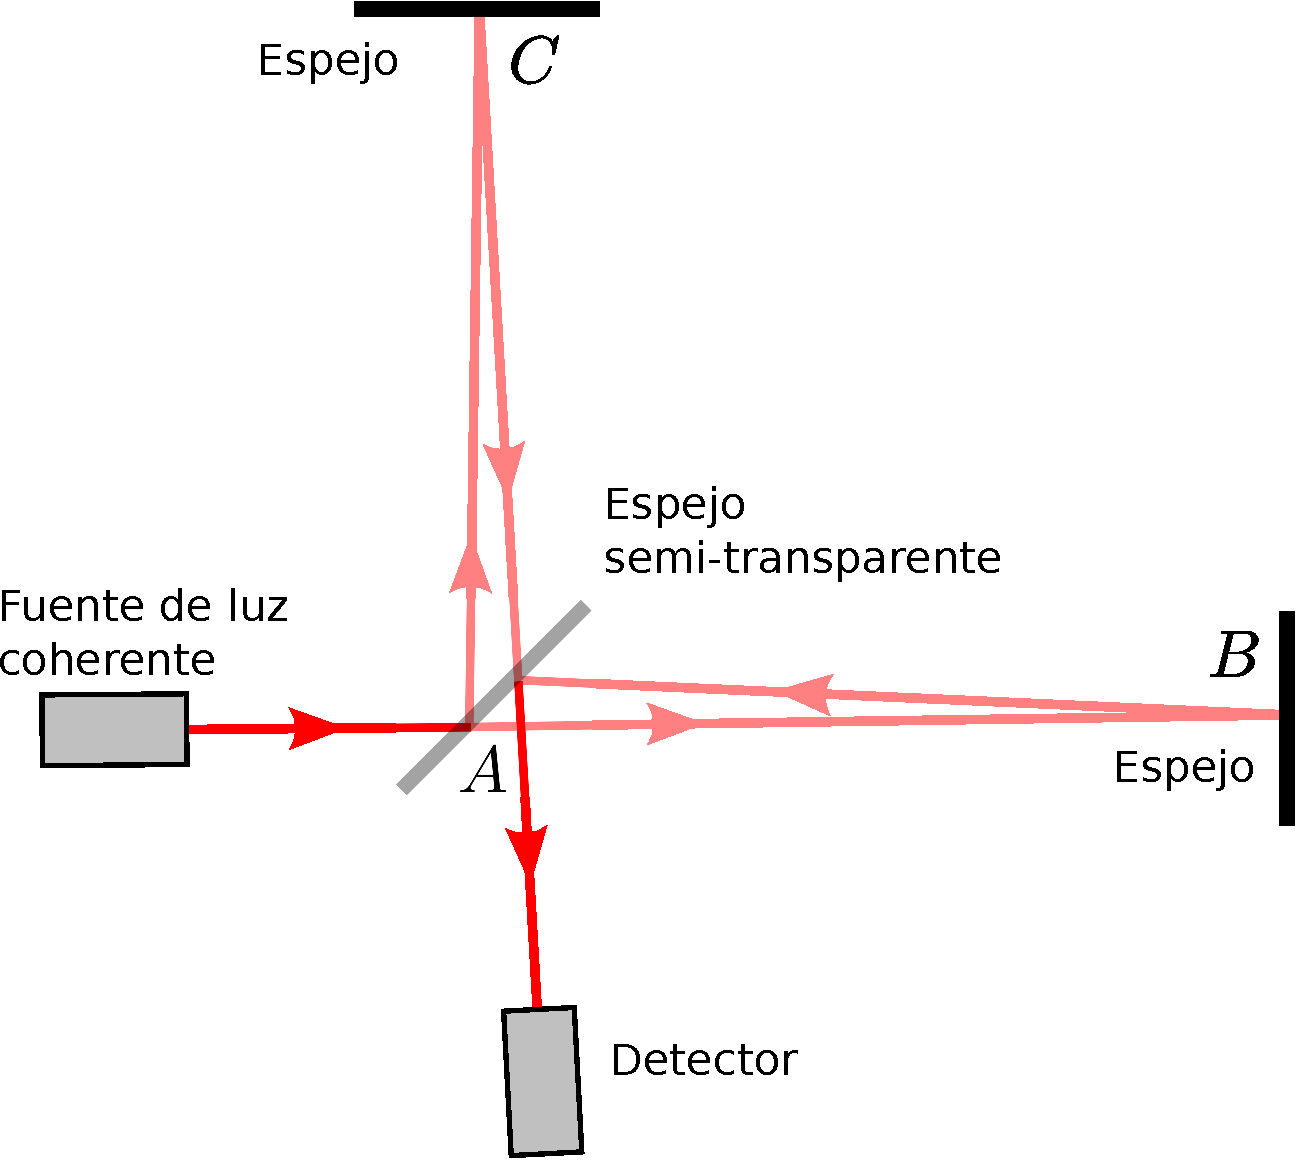
\includegraphics[width=5cm]{fig/fig-interferometro.pdf}
\end{center}
\caption{Esquema del interfer'ometro} \label{fig:michelson}
\end{figure}

Si existe alguna diferencia entre las longitudes de los brazos del interfer'ometro, aparecer'a un patr'on de interferencia. Lo mismo ocurre si los rayos se mueven a velocidades diferentes a lo largo de cada brazo. Asumiremos por simplicidad que el 'eter se mueve con velocidad $v$ a lo largo del eje $AB$.

Asumiendo que la velocidad de la luz tiene el valor conocido $c$ respecto al SR com'ovil con el 'eter entonces, de acuerdo a la mec'anica de Newton, la velocidad de la luz respecto al interfer\'ometro, en su viaje de $A$ a $B$, es $c+v$, mientras que en el viaje de regreso de $B$ a $A$, es $c-v$. Por lo tanto, el tiempo de vuelo entre de $A$ a $B$ y vuelta a $A$ es
\begin{equation} \label{eq:michelson1}
t_{ABA}=\frac{L_{AB}}{c+v}+\frac{L_{AB}}{c-v}=\frac{2L_{AB}}{c}\frac{1}{1-\beta^2},
\end{equation}
con $\beta:=v/c$. Por otro lado, el tiempo que tarda en ir de $A$ a $C$ conviene calcularlo en el SR com'ovil con el 'eter. En este caso, la propagaci'on entre $A$ y $C$ se realiza como indica la figura \ref{fig:michelson2}.
\begin{figure}[H]
\begin{center}
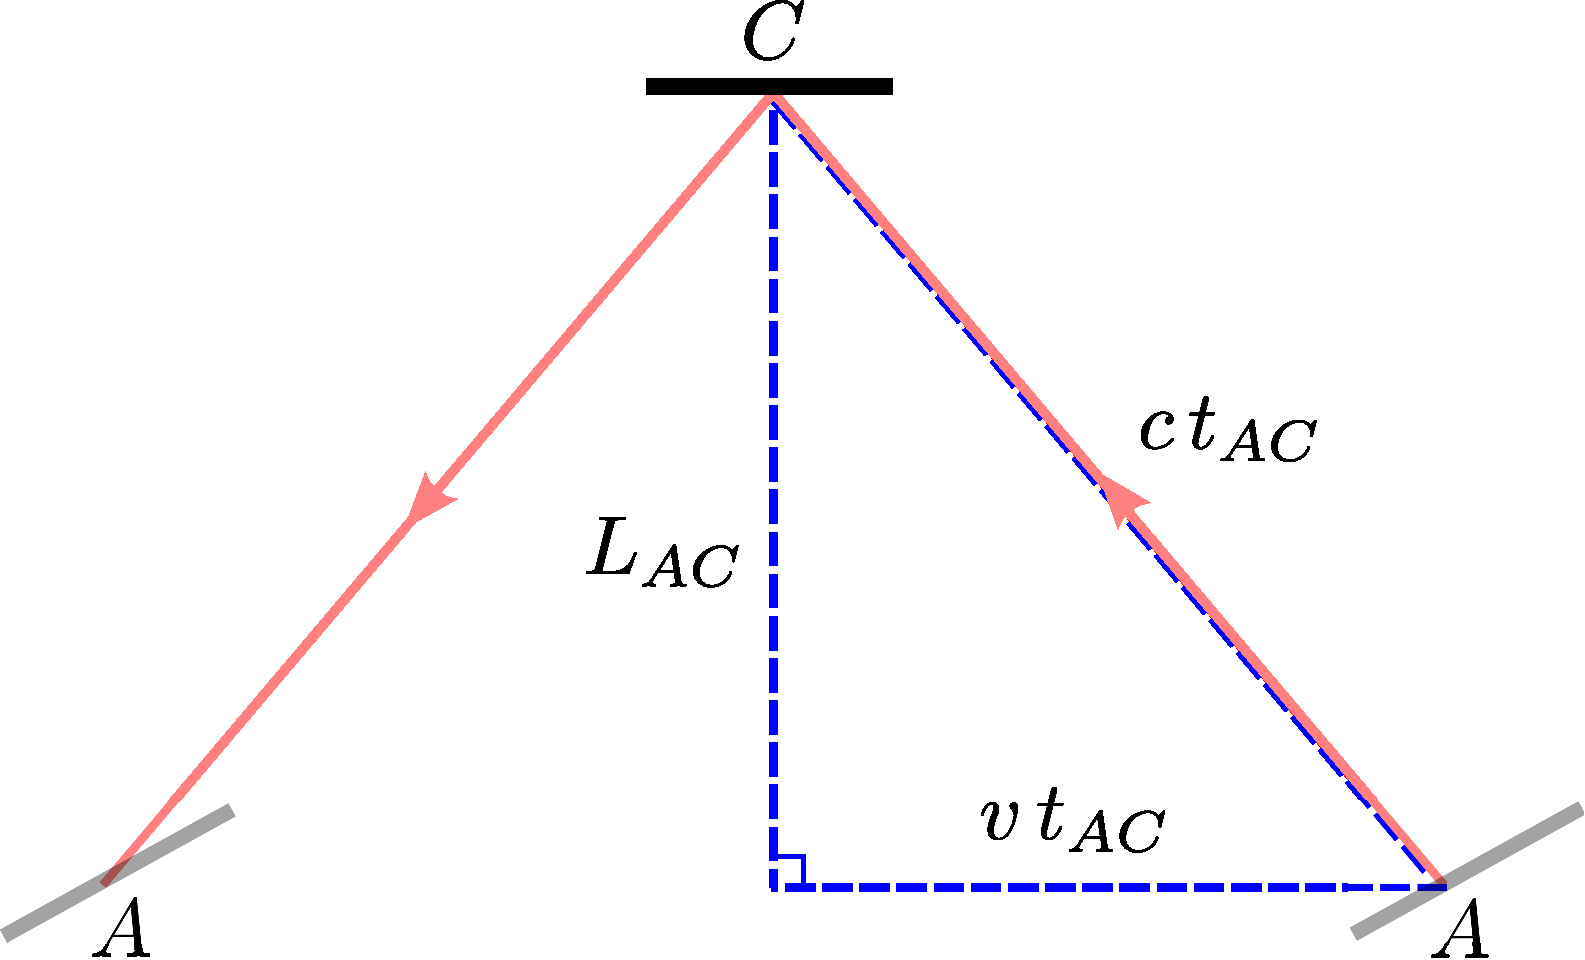
\includegraphics[width=5cm]{fig/fig-interferometro-2.pdf}
\end{center}
\caption{Propagaci'on en el segunda brazo, respecto a un SR com'ovil con el 'eter.} \label{fig:michelson2}
\end{figure}
Aplicando el teorema de Pit'agoras al tri'angulo indicado en la figura \ref{fig:michelson2} encontramos:
\begin{equation}\label{eq:michelson2}
 d^2=c^2t_{AC}^2=L_{AC}^2+(vt_{AC})^2.
\end{equation}
De aqu'i, obtenemos
\begin{equation}
 t_{AC}=\frac{L_{AC}}{c}\frac{1}{\sqrt{1-\beta^2}}
\end{equation}
y, por lo tanto,
\begin{equation} \label{eq:michelson4}
t_{ACA}=\frac{2L_{AC}}{c}\frac{1}{\sqrt{1-\beta^2}}.
\end{equation}
La diferencia de tiempos de vuelo $\Delta t:=t_{ABA}-t_{ACA}$ es entonces
\begin{equation} \label{eq:michelson5}
\Delta t=\frac{2}{c}\left[\frac{L_{AB}}{1-\beta^2}-\frac{L_{AC}}{\sqrt{1-\beta^2}}\right].
\end{equation}
Asumiendo que la velocidad del interfer'ometro respecto al 'eter es peque\~na comparada con $c$, entonces podemos expandir en potencias de $\beta$ y obtener
\begin{equation} \label{eq:michelson6}
\Delta t\approx\frac{2}{c}\left[(L_{AB}-L_{AC})+\beta^2(L_{AB}-\frac{1}{2}L_{AC})\right].
\end{equation}
An'alogamente, \textit{si se rota el interfer'ometro noventa grados}, entonces 
\begin{equation}
\Delta t'\approx\frac{2}{c}\left[(L_{AB}-L_{AC})+\beta^2(\frac{L_{AB}}{2}-L_{AC})\right].
\end{equation}

Esta diferencia de tiempo entre ambas orientaciones determina una \textit{diferencia de fase}:
\begin{equation}
\Delta\varphi=\omega(\Delta t-\Delta t')=2\pi\nu(\Delta t-\Delta t')\approx2\pi\frac{L}{\lambda} \beta^2,
\end{equation}
donde $L:=(L_{AB}+L_{AC})/2$ es la longitud efectiva de los brazos del interfer'ometro.

En el interfer'ometro usado por Michelson y Morley se usaron m'ultiples reflexiones, con el fin de aumentar el valor efectivo de $L$, de modo que $L\approx 11\,\rm m$, $\lambda\approx 5.9\times 10^{-7}\,\rm m$, $v\approx 3\times 10^4\,\rm m/s$ (la rapidez de la Tierra en su movimiento de traslaci'on en torno al Sol) y $c \approx 3\times 10^{8}\,\rm m/s$, con lo que $\Delta\varphi \approx 0,4\,\pi$, que corresponde aproximadamente a un corrimiento de \textit{media franja} en el patr'on de interferencia, que deber'ia ser posible de observar, dado el error experimental del experimento (que pod'ia detectar corrimientos de aproximadamente $0,01$ franjas).

A'un cuando el experimento se realiz'o m'ultiples veces, en diferentes 'epocas del a\~no, (y se sigue repitiendo hasta la actualidad, cada vez con mayor precisi'on, ver \cite{MHBSP03}) \textit{el experimento de Michelson-Morley arroja un resultado nulo}, es decir, ninguna variaci'on \textit{observable} del patr'on de interferencia al variar la orientaci'on del interfer'ometro respecto al 'eter.

Resumiendo: el experimento de Michelson-Morley, realizado con la intensi'on de detectar variaciones de la velocidad de la luz respecto al 'eter y de esta forma poder determinar aquel SR especial en el que la velocidad de la luz es $c$, no suministra los resultados esperados. En otras palabras, la nula variaci'on de las franjas de interferencia \textit{impide distinguir f'isicamente }(dentro del error experimental) aquel supuesto SR en el que el 'eter est'a en reposo y la luz parece propagarse con una velocidad independiente del estado de movimiento del interfer'ometro.

Se intent'o explicar el nulo resultado del experimento de Michelson-Morley manteniendo la teor'ia del 'eter y la mec'anica newtoniana. Por ejemplo, Lorentz y FitzGerald\footnote{\href{{http://es.wikipedia.org/wiki/George_Francis_FitzGerald}}{George Francis FitzGerald} (1851-1901): f'isico irland'es.} propusieron independientemente que el resultado nulo del experimento de Michelson-Morley pod'ia ser explicado asumiendo que el brazo del interfer'ometro orientado en la direcci'on del movimiento respecto al 'eter se contra'ia de modo que su longitud ser'ia $L'_{AB}=L_{AB}\sqrt{1-\beta^2}$. Lorentz también investigó la forma que debiesen tener las transformaciones de coordenadas entre dos sistemas de referencia de modo que las ecuaciones de Maxwell (y por lo tanto, sus predicciones) resultaran inalteradas. Se encontró que esto ocurre sólo si además de la contracción de Fitzgerald, se agrega una transformación de la variable temporal. Sin embargo, ninguno de estos intentos condujo a una descripci'on completa y consistente. En 1905, Albert Einstein propuso su teor'ia de la Relatividad Especial, que asumir'ia como \textit{principio} que la velocidad de la luz tiene el \textit{mismo valor en todo SRI}, m'as a'un, la \textit{equivalencia de todos los SRI's}. Einstein adem'as propuso que \textit{la luz se propaga en el vac'io}, desechando la idea del 'eter lumin'ifero. Estos postulados, sin embargo, requieren cambiar los conceptos establecidos (``newtonianos'') de distancias y tiempos.

\section{Principios de la Teor'ia de Relatividad Especial}
Einstein construy'o la teor'ia de la Relatividad Especial (RE) adoptando como postulados \textit{i}) el Principio de Relatividad, es decir, la equivalencia completa (\textit{incluyendo fen'omenos electromagn'eticos}) entre SRI's,  y \textit{ii}) el principio de constancia de la velocidad de la luz.

Antes de revisar el contenido f'isico de estos principios, introduciremos algunos conceptos b'asicos. Comenzaremos con los conceptos de \textbf{evento} y \textbf{espaciotiempo}.

Llamaremos \textbf{evento} a ``algo'' que ocurre en una regi'on limitada del
espacio en un corto intervalo de tiempo. \textit{Idealizamos} un evento como un \textit{punto} en el espacio y un \textit{instante} en el tiempo. Todos los procesos que ocurren en el Universo constituyen eventos o conjunto de eventos.
El conjunto de \textit{todos} los eventos en el Universo forma lo que
denominamos \textbf{espaciotiempo}. Supondremos entonces que el espaciotiempo es un espacio (una \textit{variedad}) \textit{cuadridimensional}.

Ilustraremos los eventos en un \textbf{diagrama de espaciotiempo}. Por ejemplo, un cuerpo con movimiento en una dimensi'on, ver figura \ref{TER1}. La curva que representa la secuencia de eventos que constituyen la ``historia'' de un cuerpo es llamada \textbf{l'inea de mundo}.

\begin{figure}[!h]
\centerline{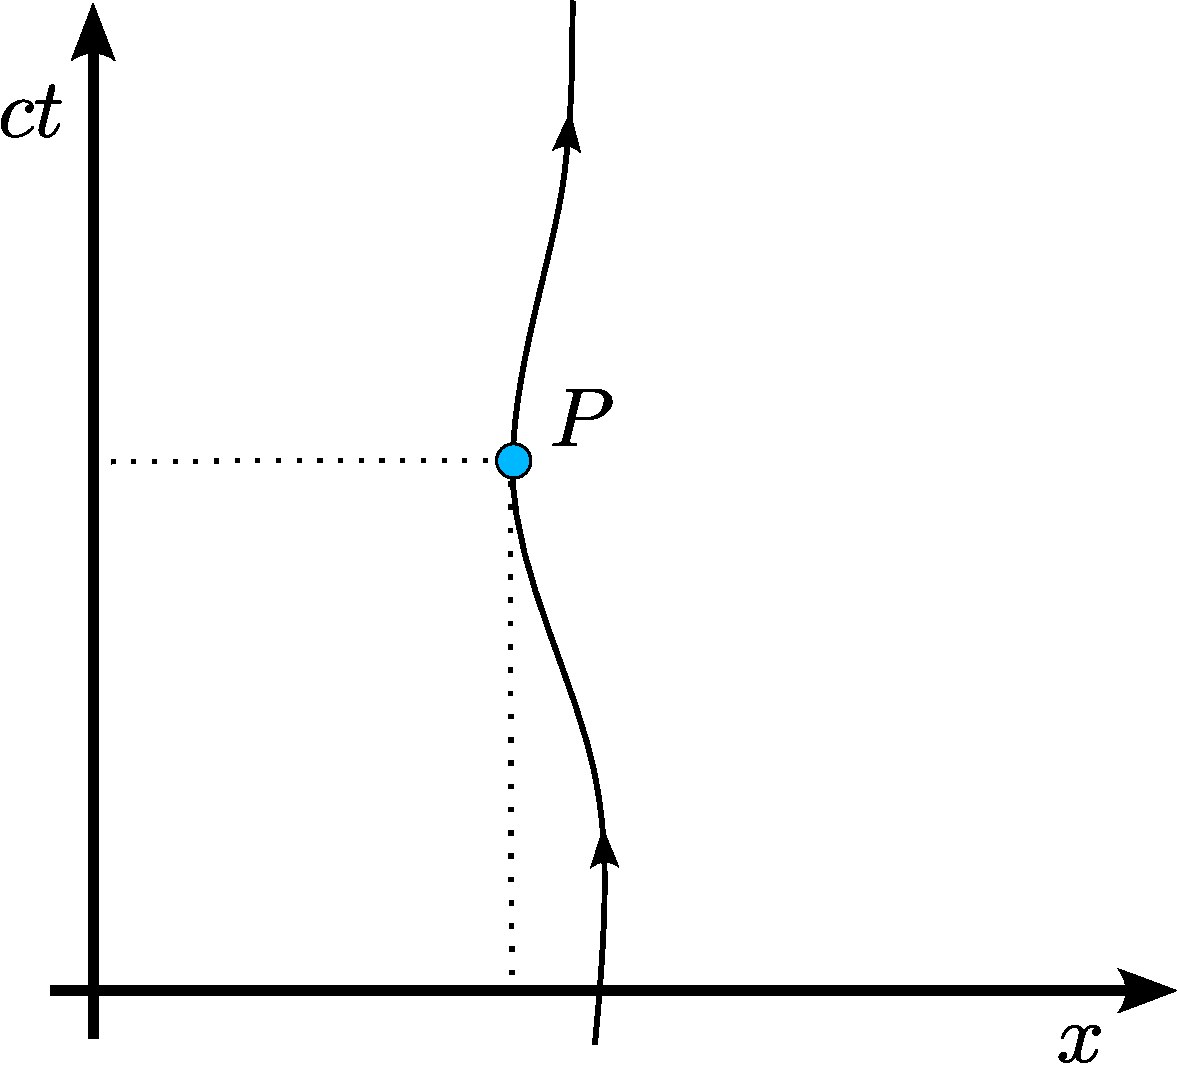
\includegraphics[height=5cm]{fig/fig-diagrama-espaciotiempo.pdf}}
\caption{Diagrama de espaciotiempo. L'inea de mundo de una part'icula.}
\label{TER1}
\end{figure}

\subsection{Principio de Relatividad}
\begin{quotation}
\ovalbox{Todos los sistemas de referencia inerciales (SRI's) son equivalentes.}
\end{quotation}

Recu'erdese que un SRI es aquel con respecto al cual un cuerpo \textit{sobre el que no act'uan agentes externos (fuerzas)} se mueve en l'inea recta a velocidad
constante.


\subsection{Principio de la constancia de la velocidad de la Luz}
 \begin{quotation}
\ovalbox{La velocidad (rapidez) de la luz tiene el mismo valor en todo SRI.}
\end{quotation}
M'as detalladamente, esto significa que las se\~nales luminosas se propagan, \textit{en el vac'io}, rectil\'ineamente con la misma rapidez ($=:c$) en todo instante, en todas direcciones, en todos los SRI's, independiente del movimiento de sus fuentes. El resultado del experimento de Michelson-Morley es consistente con el principio de constancia de la velocidad de la luz.

Adem'as, se asume que la interacci'on electromagn'etica (``la luz'') se propaga a la \textit{m'axima velocidad posible}. En otras palabras, no existe una se\~nal (m'as rigurosamente, una forma de propagar energ'ia) conocida que viaje con mayor rapidez que la luz.

Es importante descatar que la existencia de una velocidad m'axima (finita!) de las interacciones es \textit{incompatible con el concepto de
cuerpo r'igido}, puesto que 'este es, por definici'on, un objeto ideal
que no sufre deformaciones que alteren sus dimensiones (largo, ancho, ...).
Esta propiedad, sin embargo, requiere de la propagaci'on \textit{instant'anea} de interacciones en el interior del cuerpo. Es necesario, por tanto, desechar el concepto de ``cuerpo
r'igido''. Esto, por otra parte, obliga a desechar el concepto de ``regla
est\'andar'', que es (era) en el contexto newtoniano frecuentemente usado para definir patrones de longitud (metro patr'on, etc.).

Por lo tanto, en la teor'ia de RE, la existencia de una velocidad m'axima de propagaci'on de las interacciones obliga a reducir el n'umero de cantidades f'isicas en principio medibles independientemente sin ambig\"uedad, eliminando en general el concepto de distancia como concepto absoluto, y a reemplazarlo por el de medidas de tiempo.

De hecho, la definici'on actual del patr'on de longitud en el Sistema
Internacional (SI), el metro, se basa en medidas de tiempo. En 1983 (en la 17a
conferencia de pesos y medidas) se acord'o que\footnote{Recuerde adem'as que, por definici'on, un segundo es ``la duraci'on de 9.192.631.770 periodos de la radiaci'on correspondiente a la transici'on entre los dos niveles hiperfinos del estado fundamental del 'atomo de Cesio 133''. Ver \href{http://physics.nist.gov/cuu/Units/current.html}{esta} p'agina del NIST para un resumen de las unidades en el S.I. e informaci'on de la historia asociada a cada unidad.}.
\begin{quotation}
\ovalbox{Un \textit{metro} es la distancia que la luz recorre en
$1/299792458$ segundos.}
\end{quotation}
Como una consecuencia de esta definici'on, la rapidez de la luz es hoy una
cantidad \textit{exacta} con valor
\begin{equation}
\boxed{c:=299.792.458\ m/s,}
\end{equation}
ver \cite{CODATA00}.

\subsection{Definiendo posiciones y tiempos de eventos respecto a un SRI}

Ya que no podemos recurrir a ``reglas est\'andar'', debemos revisar c'omo definimos la posici'on y el tiempo que un (observador en un) SRI asocia a un evento. En general, los 'unicos tiempos \textit{directamente medibles} son los tiempos medidos por alg'un reloj (con alg'un estado de movimiento), \textit{entre eventos sobre su propia l'inea de mundo}. Éstos son los llamados \textbf{tiempos propios} asociados a un \textit{observador com'ovil con el reloj}. Es importante convencerse que no es posible medir \textit{directamente} intervalos de tiempo entre eventos \textit{alejados} de un reloj (de un observador dado).

En general, dado un evento $P$ en el espaciotiempo, \textit{definiremos} la posici'on (distancia) y tiempo del evento con respecto a un SRI $K$ dado, usando el siguiente procedimiento:

Un(a) observador inercial (puntual) define un SRI $K$ (de modo que 'el/ella est'e  ubicado en su origen) env'iando se\~nales luminosas de modo que 'estas sean reflejadas en cada evento $P$ y vuelvan al observador. El observador dispone de un reloj,  con el que mide los tiempos de salida de la se\~nal, $T_1$
y llegada $T_2$.
\begin{figure}[!h]
\centerline{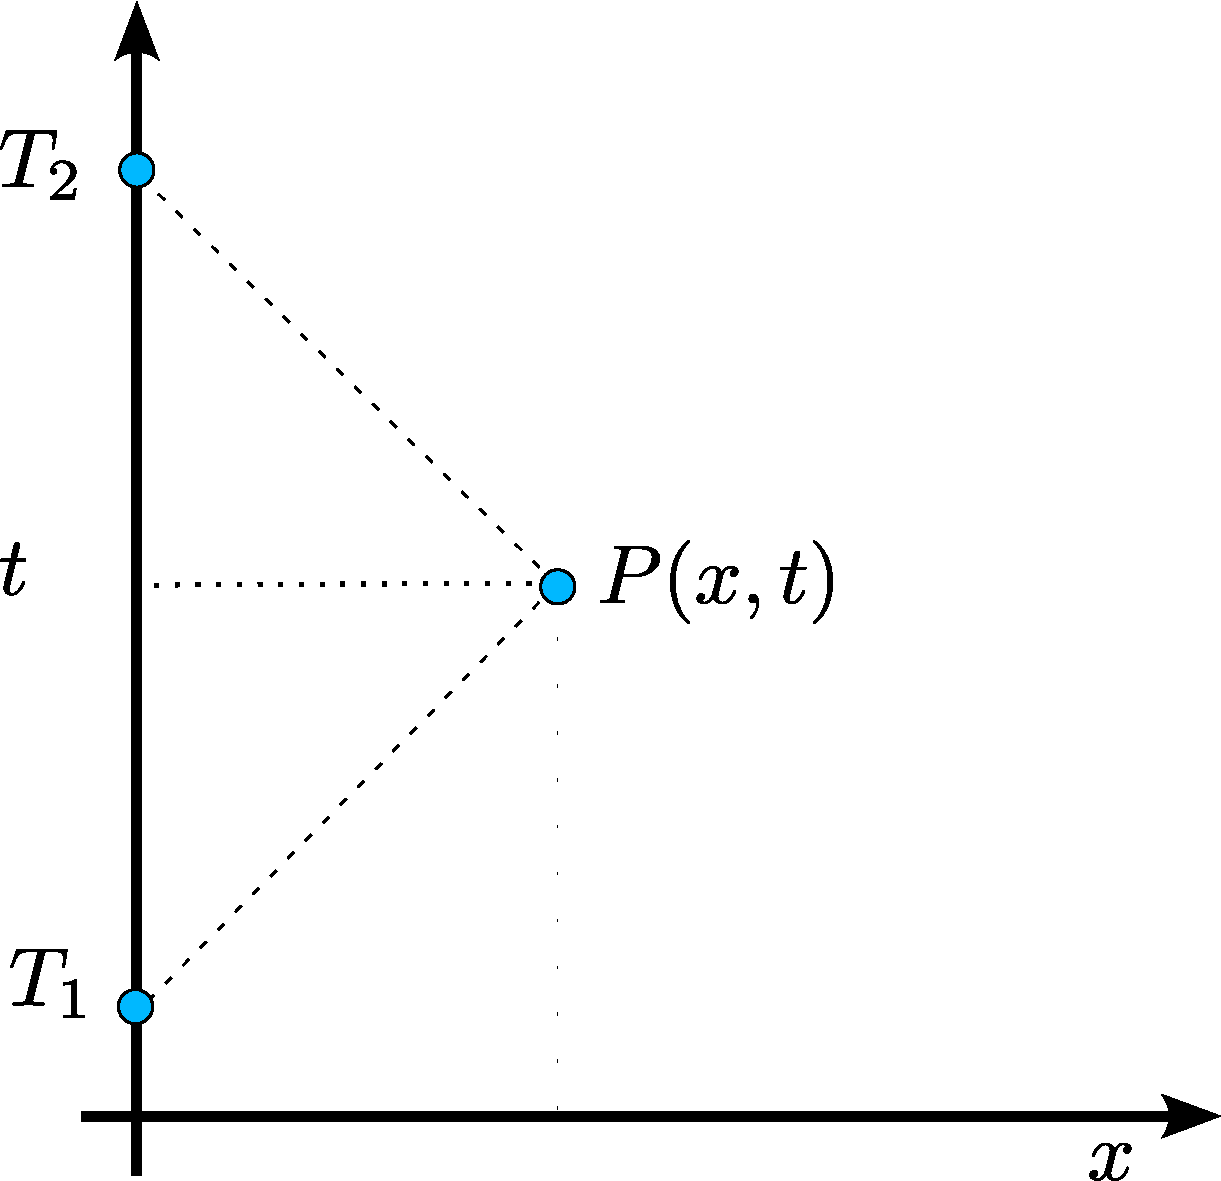
\includegraphics[height=5cm]{fig/fig-diagrama-definicion-x-y-t.pdf}}
 \caption{Definici'on de distancia en t'erminos de tiempos (propios) de vuelo.}
\label{defdist}
\end{figure}
A partir de los datos medibles (tiempos propios) $T_1$ y $T_2$, \textit{definimos} la posici'on
$x$ de $P$ respecto al observador (distancia observador - evento $P$) y el
tiempo $t$ que $K$ \textit{le asignar'a a} $P$ como:
\begin{equation}\label{defxt}
\boxed{x:=\frac{c}{2}(T_2-T_1), \qquad t:=\frac{1}{2}(T_2+T_1).}
\end{equation}

Diremos que, respecto al SRI $K$, el evento $P$ ocurri'o ``en la posici'on $x$ en el tiempo $t$''.

Las relaciones inversas a (\ref{defxt}) son las familiares expresiones
\begin{equation}\label{T1T2xt}
T_1=t-\frac{x}{c}, \qquad T_2=t+\frac{x}{c}.
\end{equation}


Es directo extender este procedimiento a mayores dimensiones (ejes $y$ y $z$), para as'i definir las coordenas $\vec{x}=(x,y,z)$ del evento $P$ respecto a cada SRI.
De este modo, podemos asociar a cada evento, respecto a un SRI, un conjunto de
coordenadas $x^\mu:=\left(ct,x,y,z\right)=(ct,\vec{x}) $.


\subsection{Relacionando mediciones de tiempo entre dos observadores inerciales}

Por simplicidad, consideraremos el caso simplificado de movimientos en
una dimensi'on.

Considere dos observadores $A$ y $B$, en reposo y movi'endose con
velocidad constante respecto a un SRI $K$, respectivamente.
\begin{figure}[H]
\centerline{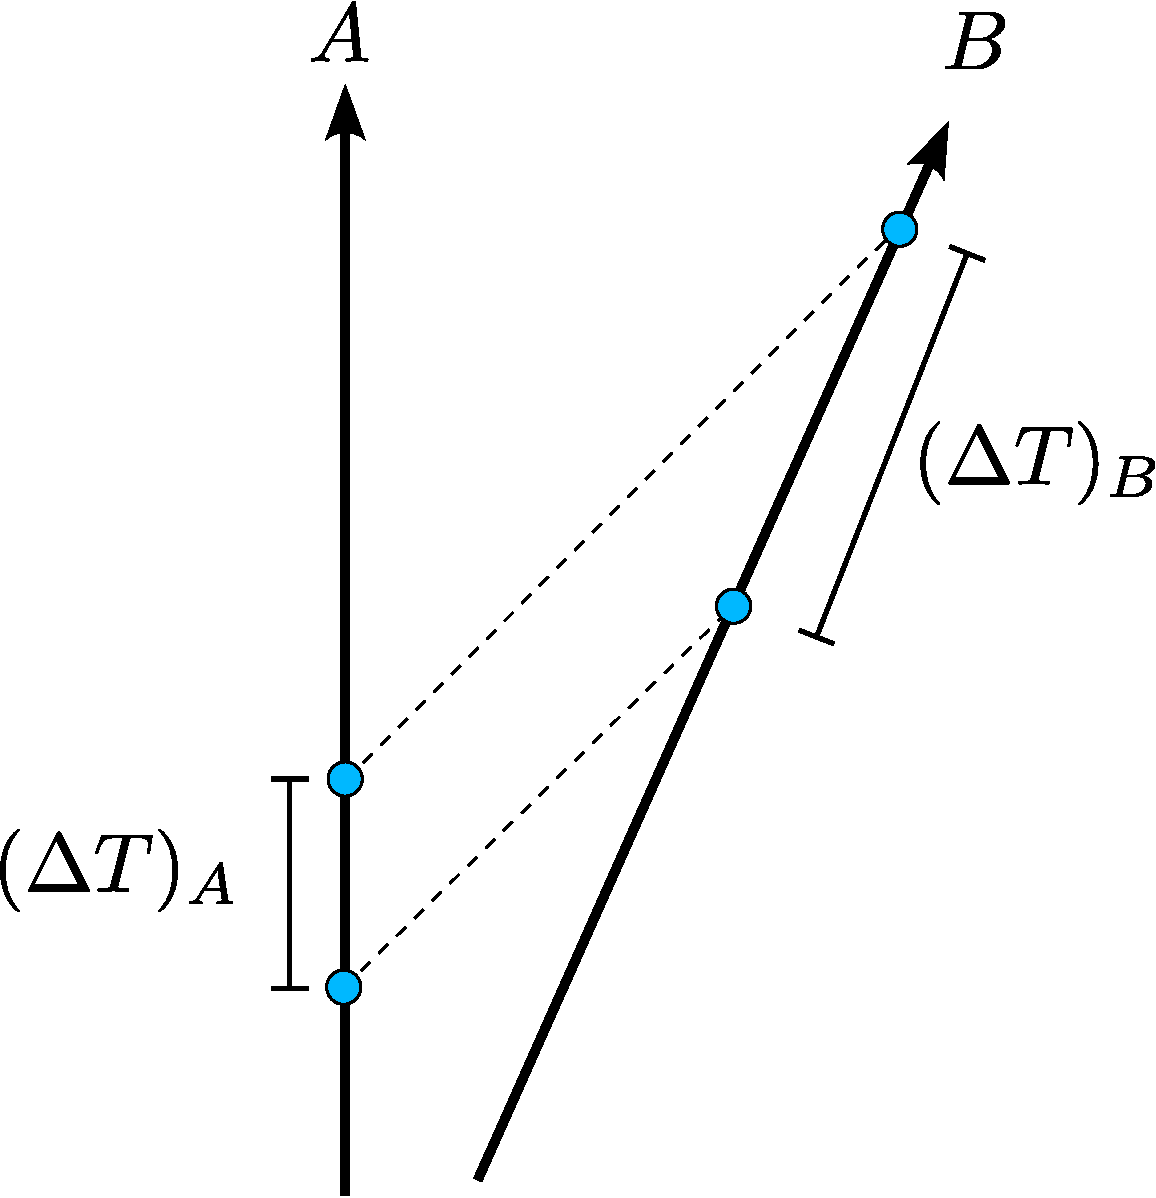
\includegraphics[height=5cm]{fig/fig-diagrama-factor-k.pdf}}
 \caption{Dos observadores inerciales intercambiando se\~nales luminosas.}
\label{k1}
\end{figure}
El observador $A$ env'ia dos se\~nales luminosas a $B$, en un intervalo de tiempo $(\Delta T)_A$, medido por $A$.

\textit{Supondremos}, como parece razonable, que el intervalo de tiempo medido por $B$ entre la llegada
de los dos pulsos, $(\Delta T)_B$, es proporcional a $(\Delta T)_A$:
\begin{equation}
(\Delta T)_B=k (\Delta T)_A. \label{TAkTB}
\end{equation}
Adicionalmente, \textit{supondremos} que:
\begin{itemize}
\item $k$ es \textit{independiente del tiempo} si $A$ y $B$ son observadores inerciales (OI's) (``homogeneidad bajo
translaciones temporales'').
\item $k$ es \textit{independiente de las posiciones} de $A$ y $B$ (``homogeneidad bajo translaciones'').
\item $k$ es \textit{independiente de la orientaci'on relativa} de $A$ y $B$ (``homogeneidad bajo rotaciones'').
\end{itemize}

Por otro lado, el Principio de Relatividad exige que la relaci'on sea rec'iproca:
\begin{equation}
(\Delta T')_A=k (\Delta T')_B .\label{tkt}
\end{equation}
Note, sin embargo, que esta relaci'on involucra intervalos de tiempo de \textit{pares de eventos distintos} a los referidos en la relaci'on (\ref{TAkTB}).

\subsection{Velocidad relativa de dos observadores inerciales}

Considere dos OI's $A$ y $B$ que sincronizan sus relojes de
modo que 'estos marquen cero en el evento com'un $O$, y que adem'as intercambian se\~nales luminosas, tal como se ilustra en la figura \ref{fig:k2}.
\begin{figure}[H]
\centerline{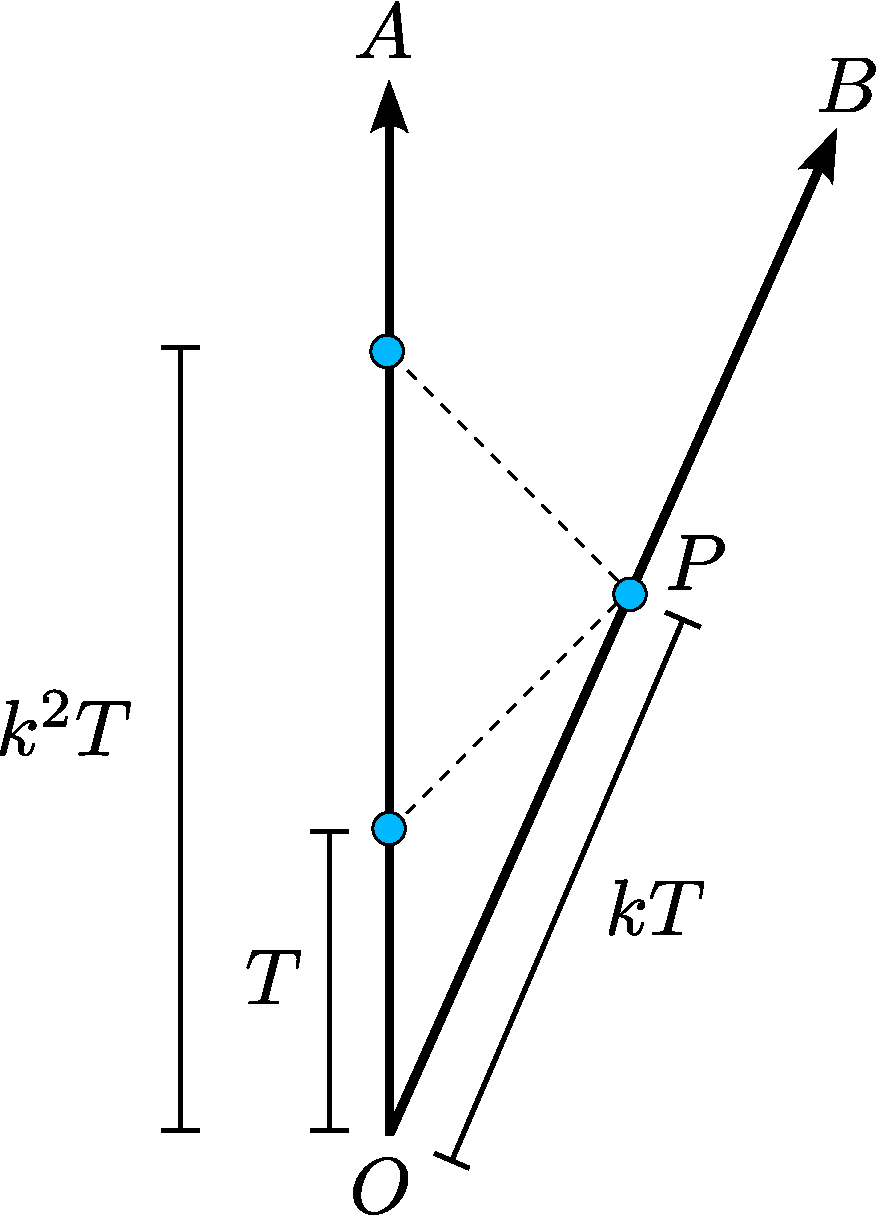
\includegraphics[height=5cm]{fig/fig-diagrama-velocidad-relativa.pdf}}
 \caption{Diagrama para determinar la velocidad relativa.}
\label{fig:k2}
\end{figure}
Nos concentraremos en las coordenadas que $A$ y $B$ asignan al evento $P$, que  pertenece a la l'inea de mundo de $B$. Las coordenadas $(t,x)$ de $P$
respecto a $A$ son
\begin{equation}
t_A(P)=\frac{1}{2}(t_1+t_2)=\frac{1}{2}(T + k^2T)=\frac{1}{2}(1+k^2)T,
\end{equation}
\begin{equation}
x_A(P)=\frac{c}{2}(k^2T-T)=\frac{c}{2}(k^2-1)T.
\end{equation}
A medida que $T$ cambia, las coordenadas del punto $P$, $t_A(P)$ y $x_A(P)$, definen la trayectoria de $B$ respecto de $A$. Por tanto, podemos calcular la \textit{velocidad de $B$ respecto de $A$} como
\begin{equation}
v_{BA}:=\frac{dx_A}{dt_A}(P)=\frac{c(k^2-1)}{1+k^2}.
\end{equation}
Despejando $k_{AB}$ obtenemos
\begin{equation}
k_{AB}=\sqrt{\frac{1+\frac{v_{BA}}{c}}{1-\frac{v_{BA}}{c}}} \,.\label{k}
\end{equation}

Con esto, la relaci'on (\ref{TAkTB}) puede escribirse como
\begin{equation}
(\Delta T)_B=\sqrt{\frac{1+\frac{v_{BA}}{c}}{1-\frac{v_{BA}}{c}}}
\,(\Delta T)_A. \label{k2}
\end{equation}
Observe que esta relaci'on es \textit{universal} en el sentido que conecta los intervalos de tiempo de cada par de eventos en la l'inea de mundo de dos observadores inerciales, siempre que 'estos est'en conectados por se\~nales luminosas, tal como lo muestra la figura \ref{k1}.

En particular, podemos aplicar esta relaci'on al caso en que $(\Delta T)_A$ y
$(\Delta T)_B$ son los \textit{periodos de una onda electromagn'etica} que se propaga de $A$ a $B$. En este caso, podemos reescribir (\ref{tkt}) en t'erminos de la \textit{frecuencia} de la radiaci'on:
\begin{equation}
\nu_B=\nu_A\sqrt{\frac{c-v_{BA}}{c+v_{BA}}},
\end{equation}
que es la expresi'on relativista para el cambio de frecuencia debido al movimiento relativo (efecto Doppler). Vemos entonces que:
\begin{itemize}
\item Si $v_{BA}>0$ (alej'andose), entonces $k_{AB}>1$, $\nu_B <
\nu_A$.
Tenemos un corrimiento hacia el rojo (\textit{redshift}).
\item Si $v_{BA}<0$ (acerc'andose), entonces $k_{AB}<1$, $\nu_B >
\nu_A$.
Tenemos un corrimiento hacia el azul (\textit{blueshift}).
\item Si $v_{BA}$ es reemplazado por $-v_{BA}$, entonces $k_{AB}$ es reemplazado
por $1/{k_{AB}}$, y $\nu_A$ por $\nu_B$, respectivamente.
\end{itemize}
Es com'un en aplicaciones definir el \textit{redshift} $z$ por
\begin{equation}
z:=\frac{\nu_A}{\nu_B}-1.
\end{equation}
Podemos verificar que si $|v_{BA}|\ll c$ entonces 
\begin{equation}
z=\frac{v_{BA}}{c}+O(\frac{v_{BA}^2}{c^2}),
\end{equation}
de modo que se recupera la conocida relaci'on no-relativista.

\subsection{Composici'on de velocidades}

Considere tres observadores inerciales $A$, $B$ y $C$ que intercambian se\~nales
luminosas como en la figura \ref{k3}.
\begin{figure}[!h]
\centerline{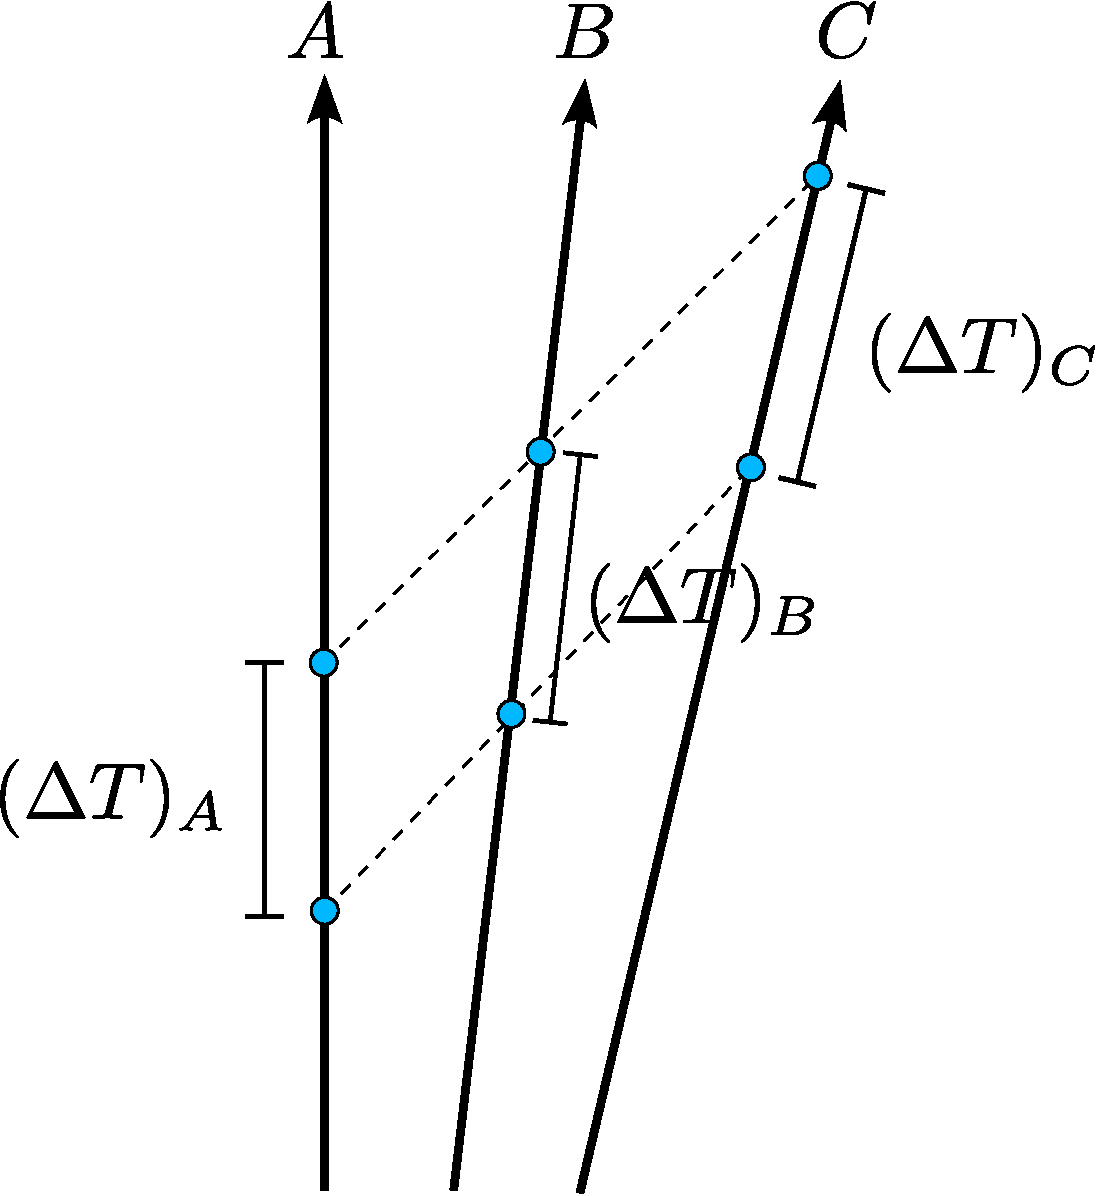
\includegraphics[height= 5cm]{fig/fig-diagrama-composicion-velocidades.pdf}}
 \caption{Tres observadores inerciales: composici'on de velocidades.}
\label{k3}
\end{figure}
 Entonces tenemos que
\begin{equation}
(\Delta T)_B=k_{AB} (\Delta T)_A, \qquad (\Delta T)_C=k_{BC} (\Delta T)_B,
\qquad (\Delta T)_C=k_{AC} (\Delta T)_A.
\end{equation}
De aqu'i obtenemos que
\begin{equation}
k_{AC}=k_{AB}k_{BC}.\label{kkk}
\end{equation}
Finalmente, usando las expresiones respectivas de los factores $k$ en funci'on
de las velocidades relativas $v_{CA}$, $v_{BA}$ y $v_{CB}$, es decir,
\begin{equation}
k_{AB}=\sqrt{\frac{1+\frac{v_{BA}}{c}}{1-\frac{v_{BA}}{c}}}, \qquad k_{BC}=\sqrt{\frac{1+\frac{v_{CB}}{c}}{1-\frac{v_{CB}}{c}}} , \qquad k_{AC}=\sqrt{\frac{1+\frac{v_{CA}}{c}}{1-\frac{v_{CA}}{c}}},
\end{equation}
en (\ref{kkk}), encontramos
\begin{equation}
\boxed{v_{CA}=\frac{v_{BA}+v_{CB}}{1+\frac{v_{BA}v_{CB}}{c^2}}.} \label{compvel}
\end{equation}

Esta \textit{ley relativista de composici'on de velocidades} (v'alida para un movimiento unidimensional) establece una \textit{velocidad absoluta}, la
velocidad de la luz. En efecto, si por ejemplo $v_{CB}=c$ (m'as rigurosamente, en el \textit{l'imite} $v_{CB}\to c$), entonces $v_{CA}=c$ independientemente del valor de $v_{BA}$. Este resultado es consistente con (en realidad, es una \textit{consecuencia de}) nuestro postulado que la velocidad de la luz tiene el mismo valor con respecto a todo SRI. Adem'as, puede verificarse [h'agalo!] que si $|v_{BA}|<c$ y $|v_{CB}|<c$, entonces  (\ref{compvel}) implica que $|v_{CA}|<c$. En otras palabras, la ley relativista de composici'on de velocidades preserva el hecho que la velocidad de los objetos (reales) siempre es menor que la velocidad de la luz, independiente del SRI respecto al cual se determine esta velocidad. Note que esto \textit{no} ocurr'ia en la teor'ia newtoniana.

% Por tanto, existen tres clases de part'iculas que en principio podr'ian existir:
% \begin{itemize}
% \item Part'iculas con $v>c$: \textit{subluminales}. Todas las part'iculas
% masivas conocidas ($e^-$, $n$, \dots).
% \item Part'iculas con $v=c$: \textit{luminales}. Todas las part'iculas sin
% masa conocidas ($\gamma$, antes tambi'en el $\nu$).
% \item Part'iculas con $v>c$: \textit{superluminales}. Ninguna conocida (violan
% causalidad), se denominan genericamente \textit{takiones}.
% \end{itemize}


\subsection{Experimento de Fizeau*}
La ley relativista de composici'on de velocidades explica muy simplemente el
resultado del experimento de Fizeau (1851), quien midi'o con t'ecnicas
interferom'etricas, la velocidad de propagaci'on de la luz \textit{en el agua}
y su dependencia con la velocidad del agua.
\begin{figure}[!h]
\centerline{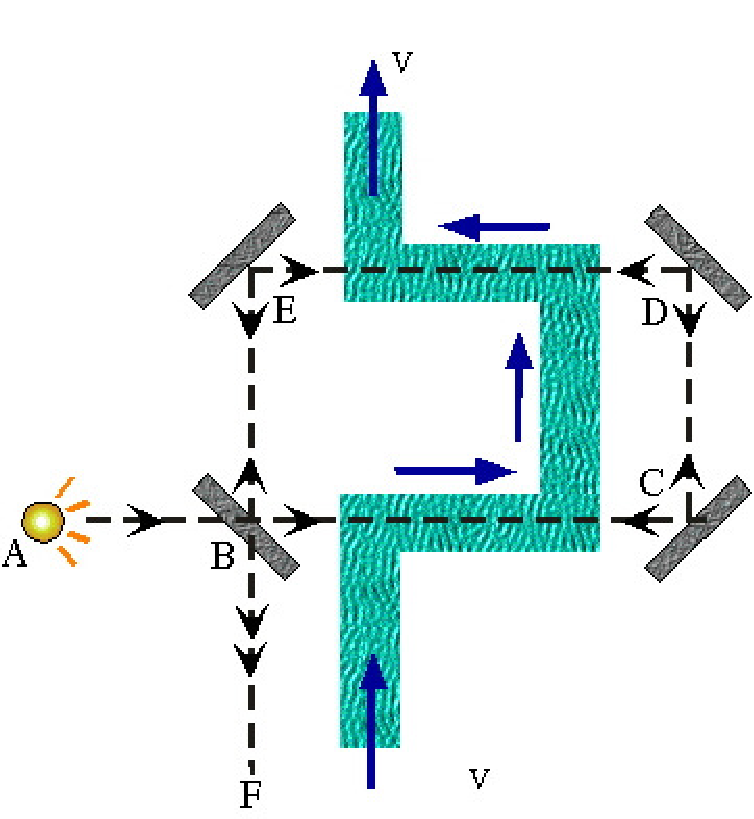
\includegraphics[height=5cm]{fig/fig-fizeau.pdf}}
 \caption{Diagrama del interfer'ometro de Fizeau}
\label{fizeau}
\end{figure}
'El encontr'o que la velocidad de la luz respecto al agua es dada por
\begin{equation}
v'=\frac{c}{n}-\left(1-\frac{1}{n^2}\right)v_{\rm agua} ,
\end{equation}
donde $n$ es el 'indice de refracci'on del agua, movi'endose con velocidad $v_{\rm agua}$.

Esta expresi'on puede ser obtenida, a segundo orden, de (\ref{compvel}) con
$v_{CA}=v'$, $v_{BA}=-v_{\rm agua}$ y $v_{CB}=c/n$ como la velocidad de la luz
respecto del agua en movimiento, del agua en reposo respecto al agua en
movimiento y de la luz respecto al agua en reposo, respectivamente ($A=$ agua
en movimiento, $B=$ agua en reposo, $C=$ luz):
\begin{equation}
v'=\frac{-v_{\rm agua}+\frac{c}{n}}{1-\frac{v_{\rm
agua}}{nc}}=\left(\frac{c}{n}-v_{\rm agua}\right)\left(1+\frac{v_{\rm
agua}}{nc}+O(\frac{v_{\rm agua}^2}{c^2})\right)=\frac{c}{n}-v_{\rm
agua}+\frac{v_{\rm agua}}{n^2}+O(\frac{v_{\rm
agua}^2}{c^2}).
\end{equation}
Antes de la formulaci'on de la teor'ia especial de la relatividad, los
resultados de este experimento se explicaban asumiendo que el agua en movimiento
``arrastraba'' parcialmente al 'eter, en una fracci'on ad-hoc.


\subsection{Boosts de Lorentz} \label{secboostx}
\begin{figure}[!h]
\centerline{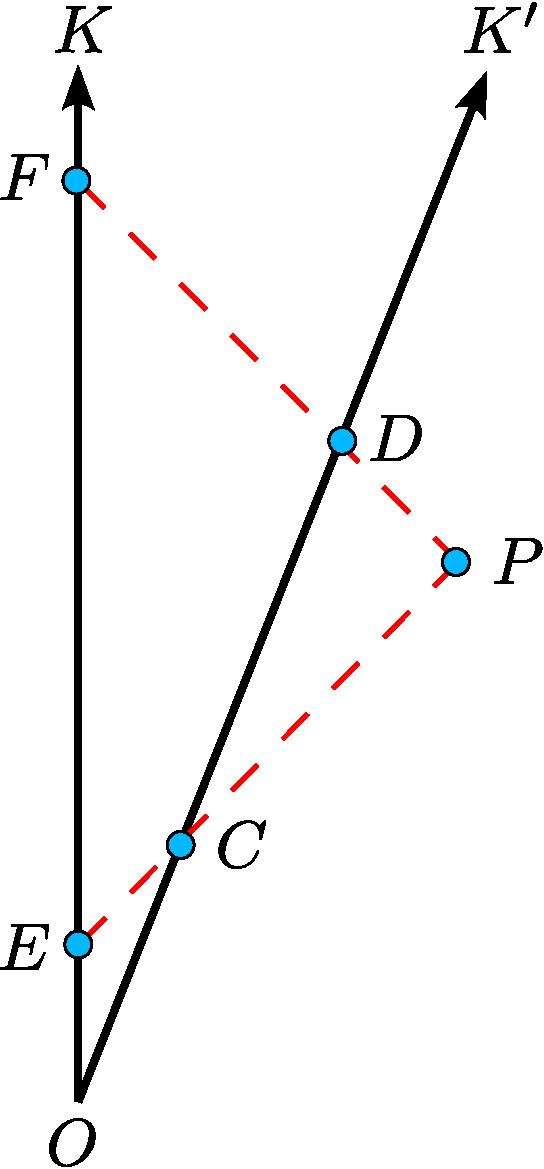
\includegraphics[height= 5cm]{fig/fig-diagrama-boost.pdf}}
 \caption{Diagrama para un boost.}
\label{boo}
\end{figure}
Ahora derivaremos la relaci'on entre las coordenadas espaciotemporales $(t,x)$
y $(t',x')$ que dos SRI's $K$ y $K'$ asocian a un \textit{mismo evento} $P$, ver figura \ref{boo}. Por simplicidad, consideraremos que $x>0$, $x'>0$.

De acuerdo a las expresiones (\ref{T1T2xt}), como $P$ tiene coordenadas $(t,x)$ respecto de $K$, entonces el evento $E$ ocurre en el tiempo (propio) $t_E=t-x/c$ respecto de $K$ y la ``respuesta'' llega en el evento $F$, con tiempo $t_F=t+x/c$. Similarmente, el evento $C$ ocurre en $t'_C=t'-x'/c$ respecto a $K'$, mientras que $D$ ocurre $t'_D=t'+x'/c$.

Si $K$ y $K'$ tienen sus relojes sincronizados cuando pasan por el evento com'un $O$, entonces tenemos, del tri'angulo $OEC$ de la figura \ref{boo}, que $t'_C=k\,t_E$, es decir,
\begin{equation}\label{rb01}
t'-\frac{x'}{c}=k\left(t-\frac{x}{c}\right),
\end{equation}
donde $k$ depende de la \textit{velocidad relativa $V$ de $K'$ respecto a $K$}:
\begin{equation}\label{kbeta}
k=\sqrt\frac{1+\beta}{1-\beta}, \qquad \beta:=\frac{V}{c}.
\end{equation}
Adem'as, del tri'angulo $ODF$ de la figura \ref{boo}, obtenemos $t_F=k\,t'_D$, es decir,
\begin{equation}\label{rb02}
t+\frac{x}{c}=k\left(t'+\frac{x'}{c}\right).
\end{equation}
Usando \eqref{rb01}, \eqref{kbeta} y \eqref{rb02} podemos despejar $x'$ y $t'$ en funci'on de $x$, $t$ y la velocidad relativa $V$ (de $K'$ con respecto a $K$), obteniendo
\begin{equation}
t'=\frac{t-\frac{Vx}{c^2}}{\sqrt{1-\frac{V^2}{c^2}}}, \qquad
x'=\frac{x-Vt}{\sqrt{1-\frac{V^2}{c^2}}}. \label{b1}
\end{equation}
Definimos el ``factor de Lorentz'' $\gamma:={1}/{\sqrt{1-\beta^ 2}}$, de modo que podemos escribir:
\begin{equation}\marginnote{Boost 1D}
\boxed{ct'=\gamma (ct-\beta x), \qquad x'=\gamma(x-\beta ct).} \label{boost1}
\end{equation}

Esta transformaci'on es conocida como un \textit{boost} (o transformaci'on de Lorentz simple) en la direcci'on $x$ y representa la transformaci'on de las coordenadas espaciotemporales \textit{de un mismo evento} desde un SRI $K$ a otro $K'$, que se mueve con velocidad $V$ con respecto al primero.

Es directo verificar que:
\begin{itemize}
\item Despejando $(t,x)$ en funci'on de $(t',x')$ se obtiene la misma
dependencia funcional que en (\ref{boost1}), pero reemplazando $V$ por $-V$, es decir,
\begin{equation}
\boxed{ct=\gamma (ct'+\beta x'), \qquad x=\gamma(x'+\beta ct').} \label{boost2}
\end{equation}
'Esta es una manifestaci'on del Principio de Relatividad.

\item Dos boosts sucesivos con velocidades $V_{BA}$ y $V_{CB}$ es
equivalente a un 'unico boost con velocidad $V_{CA}$, dada por (\ref{compvel}).

\item En el l'imite en que la velocidad de la luz fuese infinita, es decir, si la luz se propagase instant'aneamente, las transformaciones (\ref{b1}) se reducen a las \textit{transformaciones de Galileo}: $t'=t$, $x'=x-Vt$.

\item A partir de (\ref{boost1}) podemos derivar nuevamente la ley relativista de composici'on de velocidades. Si $x(t)$ es la trayectoria de una part'icula respecto al SRI $K$, entonces su velocidad es definida como $v:=dx/dt$. Similarmente, $v'=dx'/dt'$ es la velocidad respecto al SRI $K'$. Diferenciando (\ref{boost1})  obtenemos:
\begin{equation}
 v'=\frac{dx'}{dt'}=\frac{c\gamma(dx-\beta c dt)}{\gamma(cdt-\beta dx)}=\frac{c(v-\beta c)}{(c-\beta v)}=\frac{v-V}{1-\frac{V\cdot v}{c^2}}.
\end{equation}
La inversa de esta relaci'on puede nuevamente obtenerse [compru'ebelo!] sustituyendo $V$ por $-V$, es decir,
\begin{equation}
v=\frac{v'+V}{1+\frac{V\cdot v'}{c^2}},
\end{equation}
que coincide con (\ref{compvel}) (en este caso el SRI $C$ corresponde a un sistema com'ovil con la part'icula y entonces $v_{CA}=v$, $v_{BA}=V$, $v_{CB}=v'$).

\item Considere dos eventos, $P$ y $Q$, muy pr'oximos en el espaciotiempo. Sus coordenadas respecto a un SRI $K$ son $(ct,x)$ y $(ct+cdt,x+dx)$. Tanto $dx^2$ como $dt^2$ cambian sus valores de un SRI a otro, es decir,  \textit{no son invariantes bajo un boost de Lorentz} (\ref{boost1}). Esto significa que (en nuestro ejemplo unidimensional) la distancia que un SRI asocia a un par de eventos no es una cantidad absoluta en RE, y similarmente para los intervalos de tiempo entre dos eventos. Sin embargo, la combinaci'on
\begin{equation}
ds^2:=c^2dt^2-dx^2
\end{equation}
\textit{s'i es invariante} bajo (\ref{boost1}), es decir, tiene el mismo valor en cualquier SRI. En efecto, un c'alculo directo a partir de (\ref{boost1}) muestra que
\begin{equation}
ds'^2:=c^2dt'^2-dx'^2=c^2dt^2-dx^2=ds^2.
\end{equation}
En este sentido $ds^2$ es una \textit{cantidad absoluta} en la teor'ia de RE: no importa en qu'e SRI se calcule, su valor es siempre el mismo. Esta importante cantidad recibe el nombre de \textit{intervalo}. Note que en general $ds^2$ puede asumir valores positivos, negativos o nulos, dependiendo de la elecci'on de los eventos $P$ y $Q$.

En el caso de \textit{eventos sobre la trayectoria de una part'icula}, es posible encontrar una simple interpretaci'on para el valor del intervalo: ya que $ds^2$ puede calcularse en cualquier SRI y siempre se obtendr'a el mismo valor, en particular en el SRI com'ovil con la part'icula (es decir, en el SRI con respecto al cual la part'icula est'a en reposo entre $P$ y $Q$) $dx_{\rm com}=0$ y $dt_{\rm com}=d\tau$ coincide con el intervalo de \textit{tiempo propio}, ya que ser'ia el intervalo de tiempo que mide un observador que se mueve con la part'icula. Entonces $ds^2=c^2d\tau^2$. En otras palabras $d\tau=\sqrt{ds^2}/c=ds/c$ es el intervalo de tiempo propio medido por un observador que se mueve con la part'icula. Note que en estos casos $ds^2>0$.

\end{itemize}




\subsection{Relatividad de la Simultaneidad}
Consideraremos aqu'i el ejemplo cl'asico de c'omo dos eventos que son simult'aneos respecto a un SRI no lo son respecto de otro en movimiento relativo. Para ello, considere un vag'on de tren provisto de una l'ampara en su centro que en el evento $O$ emite una se\~nal luminosa hacia los dos extremos del vag'on.
\begin{figure}[H]
\centerline{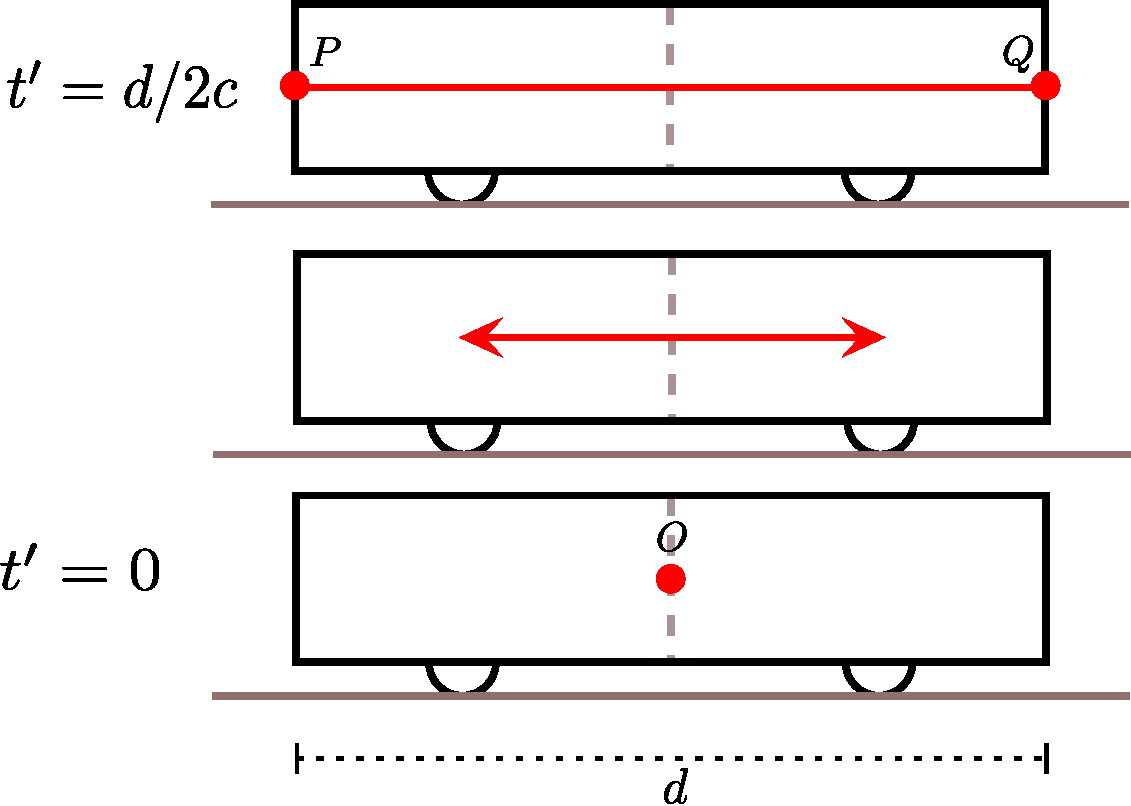
\includegraphics[height= 5cm]{fig/fig-diagrama-simultaneidad-01.pdf}}
\caption{Los eventos $P$ y $Q$ son simult'aneos respecto al SRI $K'$, com'ovil con el tren. Adaptada a partir de \href{https://commons.wikimedia.org/wiki/File:Traincar_Relativity1.svg}{esta} figura original.}
\label{sim01}
\end{figure}
En el SRI $K'$ com'ovil con el tren, el proceso transcurre como se representa en la figura \ref{sim01}\footnote{Adaptada a partir de  \href{http://commons.wikimedia.org/wiki/File:Traincar_Relativity1.svg}{esta} figura original.}. Si en este caso el largo del vag'on es $d$ y se elige el origen del tiempo tal que $t'_O=0$, entonces las se\~nales luminosas (los ``fotones'') llegan (chocan) con las paredes izquierda y derecha en los eventos $P$ y $Q$, en el mismo tiempo $t'_P=t'_Q=d/2c$. Por lo tanto, los eventos $P$ y $Q$ son simult'aneos respecto a este SRI $K'$.
\begin{figure}[H]
\centerline{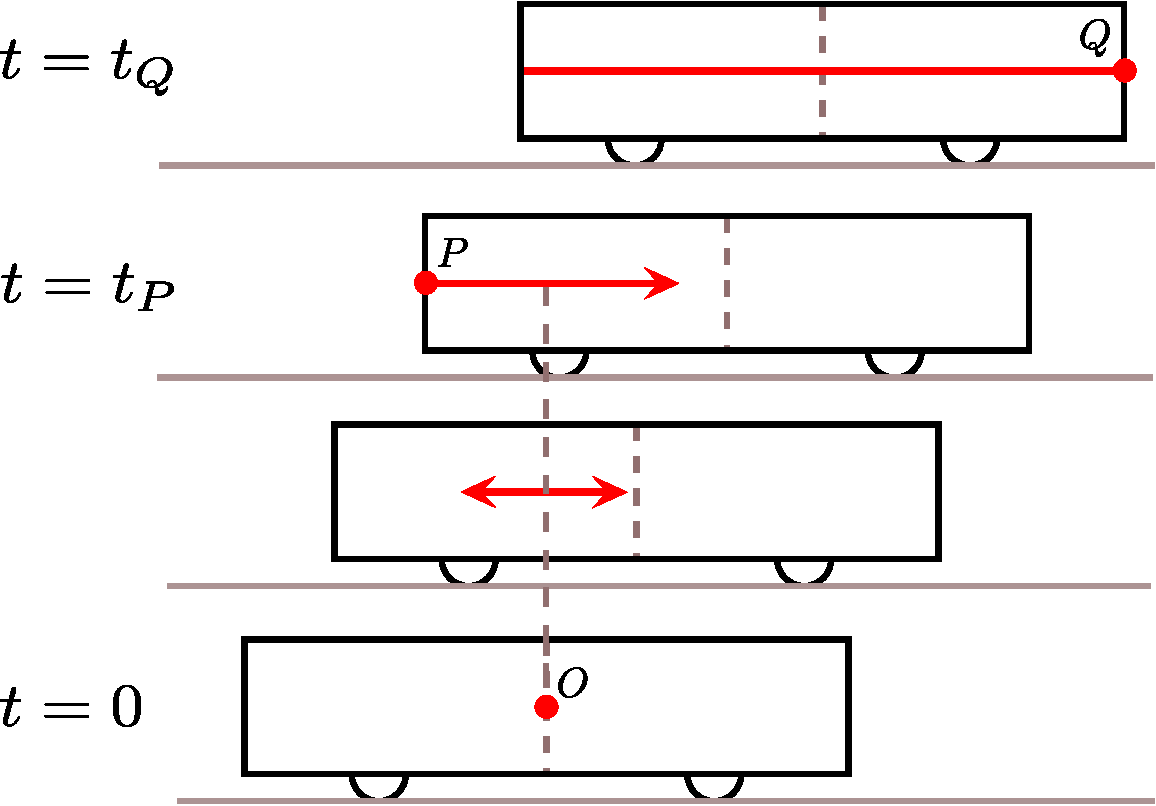
\includegraphics[height= 5cm]{fig/fig-diagrama-simultaneidad-02.pdf}}
\caption{Los eventos $P$ y $Q$ no son simult'aneos respecto al SRI $K$, respecto al cual el tren se mueve con velocidad $V$. Adaptada a partir de \href{https://commons.wikimedia.org/wiki/File:Traincar_Relativity2.svg}{esta} figura original.}
\label{sim02}
\end{figure}

Por otro lado, la descripci'on de este mismo proceso desde el SRI $K$ ``fijo a la Tierra'', respecto al cual el vag'on se mueve con velocidad $V=\beta c$, se esquematiza en la figura \ref{sim02}\footnote{Adaptada a partir de \href{http://commons.wikimedia.org/wiki/File:Traincar_Relativity2.svg}{esta} figura original.}. En este caso, la se\~nal luminosa se propaga, de acuerdo a los postulados de la teor'ia, con (la misma) velocidad $c$ hacia ambos lados. Sin embargo, las paredes del vag'on se mueven con velocidad $V$ hacia la derecha de modo que a pared izquierda se mueve hacia la se\~nal mientras que la pared derecha se aleja de ella. Claramente, en estas condiciones el evento $P$ (de intersecci'on de la l'inea de mundo de la pared izquierda con la l'inea de mundo del fot'on) ocurre \textit{antes que el evento} $Q$. Por lo tanto, respecto al SRI $K$ los eventos $P$ y $Q$ no son simult'aneos. Esto significa que, en la teor'ia de RE, \textit{la simultaneidad de eventos es relativa}.

Podemos cuantificar lo anterior usando la transformaci'on de Lorentz (\ref{boost1}). Si los observadores en $K$ y $K'$ sincronizan sus relojes en el evento $O$ en que los rayos de luz dejan el punto medio (se ``enciende la l'ampara''), entonces
\begin{eqnarray}
x'^\mu_O&=&(ct'_O,x'_O)=(0,0), \\
x'^\mu_P&=&(ct'_P,x'_P)=(d/2,-d/2), \\
x'^\mu_Q&=&(ct'_Q,x'_Q)=(d/2,d/2).
\end{eqnarray}
Usando (\ref{boost2}), encontramos que las coordenadas de estos eventos respecto al SRI $K$ son
\begin{eqnarray}
x^\mu_O&=&(ct_O,x_O)=(0,0), \\
x^\mu_P&=&(ct_P,x_P)=\left(\frac{\gamma d}{2}(1-\beta),-\frac{\gamma d}{2} (1-\beta)\right), \\
x^\mu_Q&=&(ct_Q,x_Q)=\left(\frac{\gamma d}{2}(1+\beta),\frac{\gamma d}{2} (1+\beta)\right).
\end{eqnarray}
Estas coordenadas, junto con las l'ineas de mundo de los fotones y las paredes del vag'on son representadas en la figura \ref{sim03-04}\footnote{Adaptadas a partir de \href{http://commons.wikimedia.org/wiki/File:TrainAndPlatformDiagram1.svg}{esta} y \href{http://commons.wikimedia.org/wiki/File:TrainAndPlatformDiagram2.svg}{esta} figura original.} desde el punto de vista de los SRI's $K$ y $K'$.
\begin{figure}[!h]
\centerline{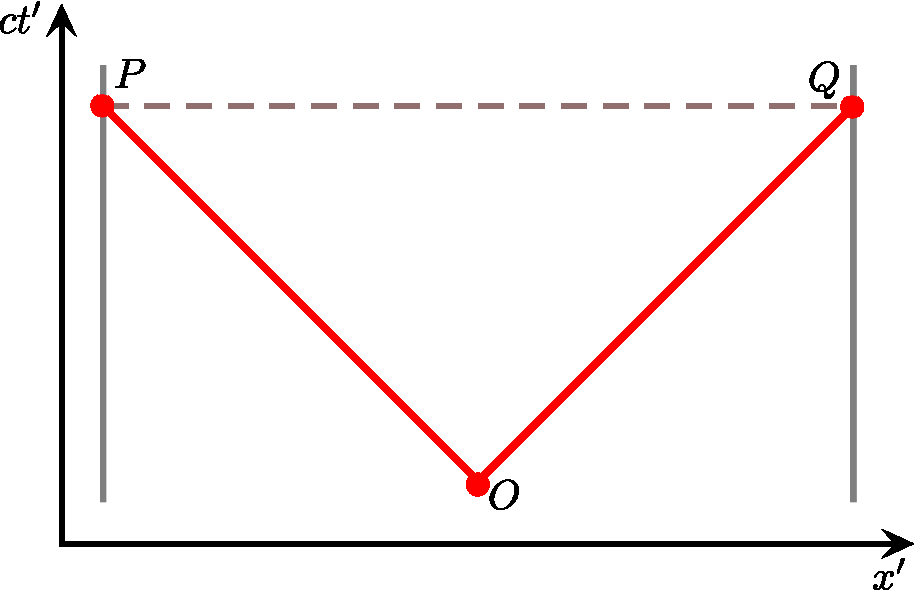
\includegraphics[height= 4cm]{fig/fig-diagrama_simultaneidad-03.pdf}\hspace{1cm}
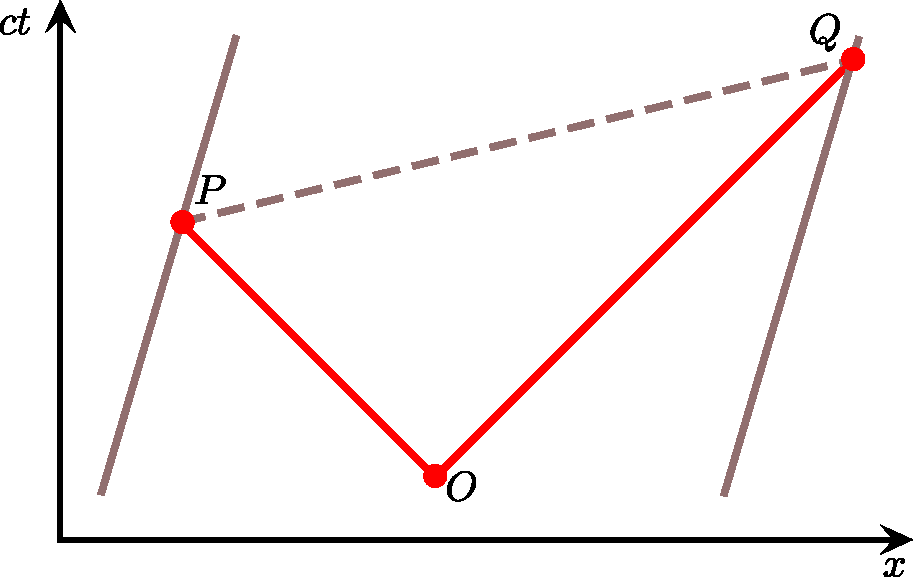
\includegraphics[height= 4cm]{fig/fig-diagrama_simultaneidad-04.pdf}}
\caption{Diagramas de espaciotiempo para el proceso, respecto a los SRI $K'$ y $K$. Adaptadas a partir de \href{https://en.wikipedia.org/wiki/File:TrainAndPlatformDiagram1.svg}{esta} y \href{https://en.wikipedia.org/wiki/File:TrainAndPlatformDiagram2.svg}{esta} figura original}
\label{sim03-04}
\end{figure}

Claramente, obtenemos $t_P<t_Q$ de modo que respecto a $K$ el evento $P$ ocurre antes que el evento $Q$. La diferencia de tiempo entre estos eventos es entonces dada por:
\begin{equation}
 \Delta t_{PQ}:=t_Q-t_P=\frac{1}{c}\gamma \beta d=\gamma\frac{V}{c^2}d >0.
\end{equation}


Por lo tanto, encontramos que respecto al SRI $K$ los eventos $P$ y $Q$ no son simult'aneos: $P$ acontece antes que $Q$ y el intervalo de tiempo entre estos dos eventos es $\gamma{V}d/{c^2}$. Similarmente, respecto a un SRI $K''$ en el que el vag'on se mueva hacia la izquierda, el evento $Q$ ocurrir'a antes que $P$. Como veremos m'as adelante, la relatividad de la simultaneidad no contradice el principio de causalidad puesto que \textit{no existe relaci'on causal entre los eventos} $P$ y $Q$.


\subsection{Dilataci'on del tiempo}
Considere dos eventos $P$ y $Q$ que, con respecto a un SRI com'ovil $K'$, ocurren en la misma posici'on, pero en tiempos diferentes. Estos mismos dos eventos ocurren en posiciones diferentes y \textit{con un intervalo de tiempo tambi'en diferente} respecto a otro SRI $K$ en movimiento relativo respecto a $K'$. 

En efecto, en este caso $(\Delta x')_{PQ}=0$ y $(\Delta t')_{PQ}=(\Delta\tau)_{PQ}\neq 0$ y por lo tanto, usando las transformaciones (\ref{boost2}) tenemos que
\begin{equation}
(\Delta t_{PQ})=\gamma (\Delta\tau)_{PQ}, \qquad (\Delta x)_{PQ}=\gamma\beta c\,(\Delta\tau)_{PQ}.
\end{equation}
De este modo encontramos que $(\Delta t)_{PQ}>(\Delta\tau)_{PQ}$, es decir, que en el SRI $K$ se asignar'a un intervalo de tiempo mayor que el que $K'$ asociar'a \textit{al mismo par de eventos}. Un ejemplo cl'asico de \textit{esta dilataci'on del tiempo} lo constituye la vida media de las part'iculas. Si la vida media de una part'icula es\footnote{Cl'asicamente la vida media de una part'icula es ``el tiempo que ella tarda en desintegrarse cu'ando est'a en reposo'' o, m'as precisamente, el tiempo que debe transcurrir para que una poblaci'on de un gran n'umero de part'iculas id'enticas y en reposo se reduzca en una fracci'on $1/e$.} $\tau_0$, entonces la vida media de ella con respecto a un observador que la ve moverse con rapidez $v$ es $\tau=\gamma\tau_0 >\tau_0$.

Esta dilataci'on del tiempo es un efecto \textit{universal} que afecta a todo tipo de eventos y en particular a la ``velocidad de avance'' de relojes en movimiento. Esto se ilustra en el siguiente ejemplo.

\subsubsection{Reloj de Luz}
Considere el ``reloj de luz'' formado por un rayo de luz que rebota entre dos espejos paralelos separados una distancia $L$, como se esquematiza en la figura\footnote{Adaptadas a partir de \href{http://en.wikipedia.org/wiki/File:Time-dilation-001.svg}{esta} y \href{http://en.wikipedia.org/wiki/File:Time-dilation-002.svg}{esta} figura original.} \ref{dt}.
\begin{figure}[!h]
\centerline{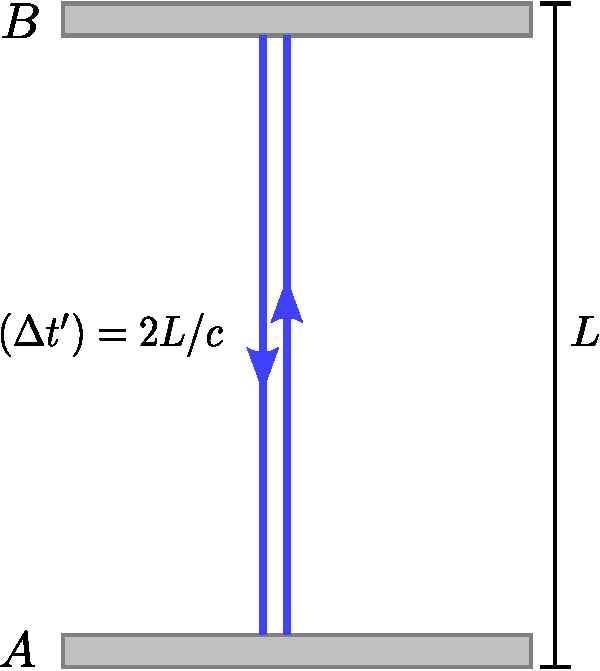
\includegraphics[height= 4cm]{fig/fig-diagrama-dilatacion-01.pdf}\hspace{1cm}
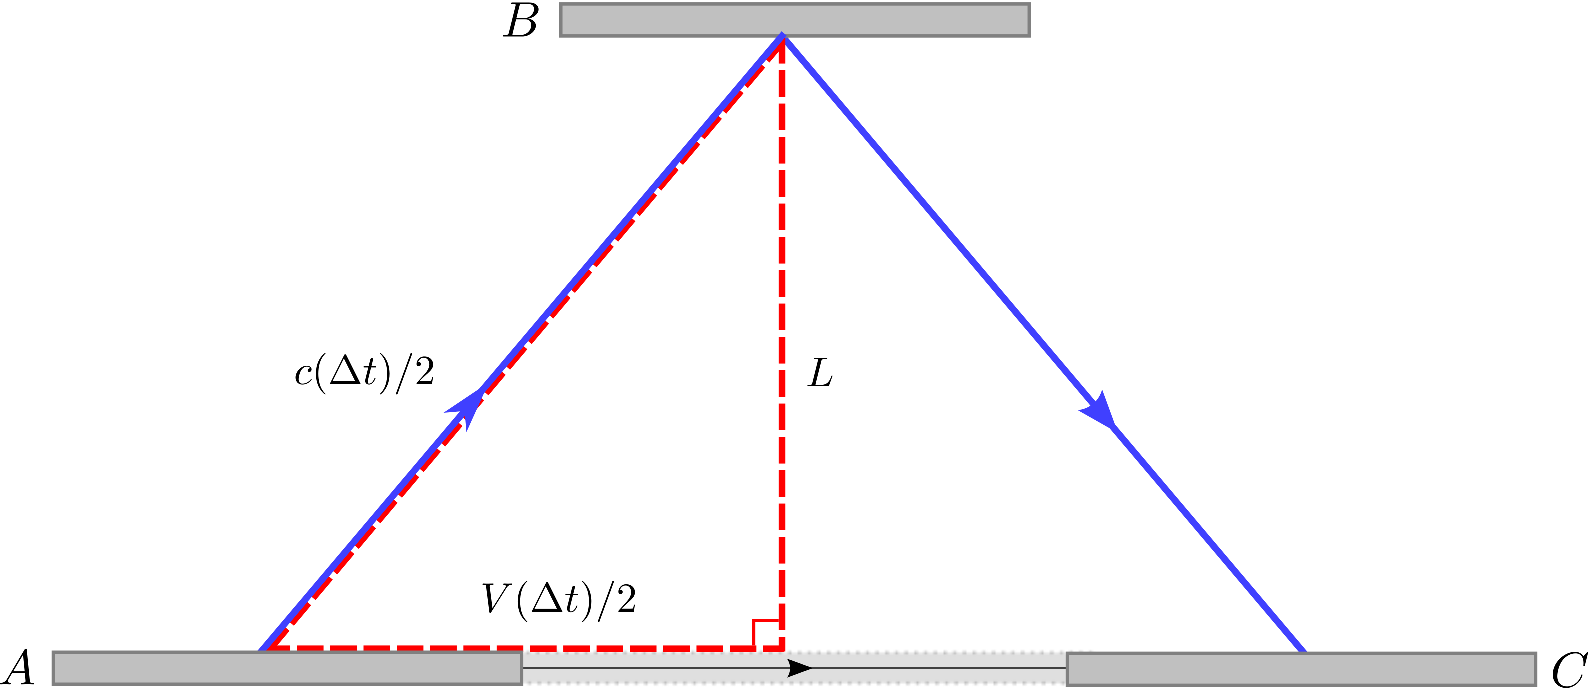
\includegraphics[height=4cm]{fig/fig-diagrama-dilatacion-02.pdf}}
 \caption{Dilataci'on del tiempo en el ``reloj de luz''. Izquierda: SRI com'ovil $K'$. Derecha SRI $K$ respecto al cual el reloj se mueve con velocidad $v=\beta c$.}
\label{dt}
\end{figure}
Respecto al SRI com'ovil $K'$ el tiempo entre la salida y la llegada del rayo de luz (un ``tic'' del reloj) es dado por
\begin{equation}
\Delta t'=\frac{2L}{c}.
\end{equation}
Por otro lado, respecto al SRI $K$ el rayo de luz tarda un tiempo $(\Delta t)$ en subir y bajar. Este tiempo puede ser determinado usando el teorema de Pit'agoras en el tri'angulo indicado en la figura:	
\begin{equation}
\left(\frac{c\Delta t}{2}\right)^2=L^2+\left(\frac{v\Delta t}{2}\right)^2.
\end{equation}
A partir de esta relaci'on, encontramos que
\begin{equation}
\Delta t=\gamma\,\Delta t'.
\end{equation}

\subsubsection{Derivaci'on usando el intervalo}

Otra forma de derivar este resultado es usando directamente el intervalo,
\begin{equation}
 ds^2=c^2d\tau^2=c^2dt^2-dx^2=c^2dt^2(1-\beta^2)=\gamma^{-2}c^2dt^2,
\end{equation}
de modo que $dt=\gamma d\tau>d\tau$.


En definitiva, \textbf{todo intervalo de tiempo que transcurre entre dos eventos dados parece mayor (dilatado) cuando se observa desde un SRI en movimiento, comparado con el intervalo de tiempo entre los mismos eventos respecto a un observador com'ovil}.

Esta predicci'on de la teor'ia de la relatividad especial ha sido confirmada experimentalmente en m'ultiples ocasiones a trav'es de mediciones del \textit{efecto Doppler (transversal)} (experimento sugerido por el mismo Einstein en 1907 \cite{Einstein07}), ya que como consecuencia de la dilatación temporal, la radiaci'on emitida por un 'atomo en movimiento transversal a la direcci'on de observaci'on, presentar'a una \textit{variación relativa de la longitud de onda} de la radiación emitida $\Delta\lambda/\lambda_0=\gamma-1\approx 10^{-5}$. La primera confirmaci'on usando este efecto es debida a Ives y Stilwell en 1938 \cite{IS38}, usando 'atomos de Hidr'ogeno  ($v/c\approx 0.005$, $\gamma-1\approx 10^{-5}$). En 2003 Saathoff et. al. publicaron resultados de un test mejorado, usando ``espectroscop'ia laser de iones r'apidos" \cite{Saathoff03} ($v/c\approx 0.064$, $\gamma-1\approx 2\times 10^{-3}$, $1\%$), y luego en 2007 Reinhardt et al. mejoraron la precisi'on usando ``relojes 'opticos at'omicos" \cite{Reinhardt07} ($v/c\approx 0.03$, $\gamma-1\approx 4\times 10^{-4}$). El ``record"\, lo tienen actualmente Chou et al., quienes lograron verificar la dilataci'on temporal con ``relojes at'omicos" (de 'atomos aluminio) moviéndose a velocidades del orden de 10 m/s ! \cite{Chou10} ($v\approx 10 [m/s]$, $v/c\approx 3\times 10^{-8}$, $\gamma-1\approx 4\times 10^{-16}$). Otros m'etodos para verificar la dilataci'on temporal consisten en medir la vida media de part'iculas \cite{Bailey77} ($v/c\approx 0.9994$, $\gamma-1\approx 28$), y comparar las medidas de relojes at'omicos en movimiento relativo (``paradoja de los gemelos'') \cite{HK72a,HK72b}. Para otras referencias sobre la confirmaci'on experimental de la teor'ia de Relatividad Especial, ver \cite{SRexp}.

\subsection{Contracci'on de la longitud}
Considere un cuerpo, cuyos extremos est'an, respecto a un SRI $K'$ com'ovil, fijos en las posiciones $x'_P$ y $x'_Q=x'_R$. Respecto a este SRI la longitud del cuerpo es $L_0=x'_Q-x'_P$. En otro SRI, respecto al cual el cuerpo se mueve con velocidad $v$, \textit{se define} la longitud $L$ como \textit{la distancia entre las posiciones de los puntos extremos del cuerpo en el mismo instante}.
\begin{figure}[!h]
\centerline{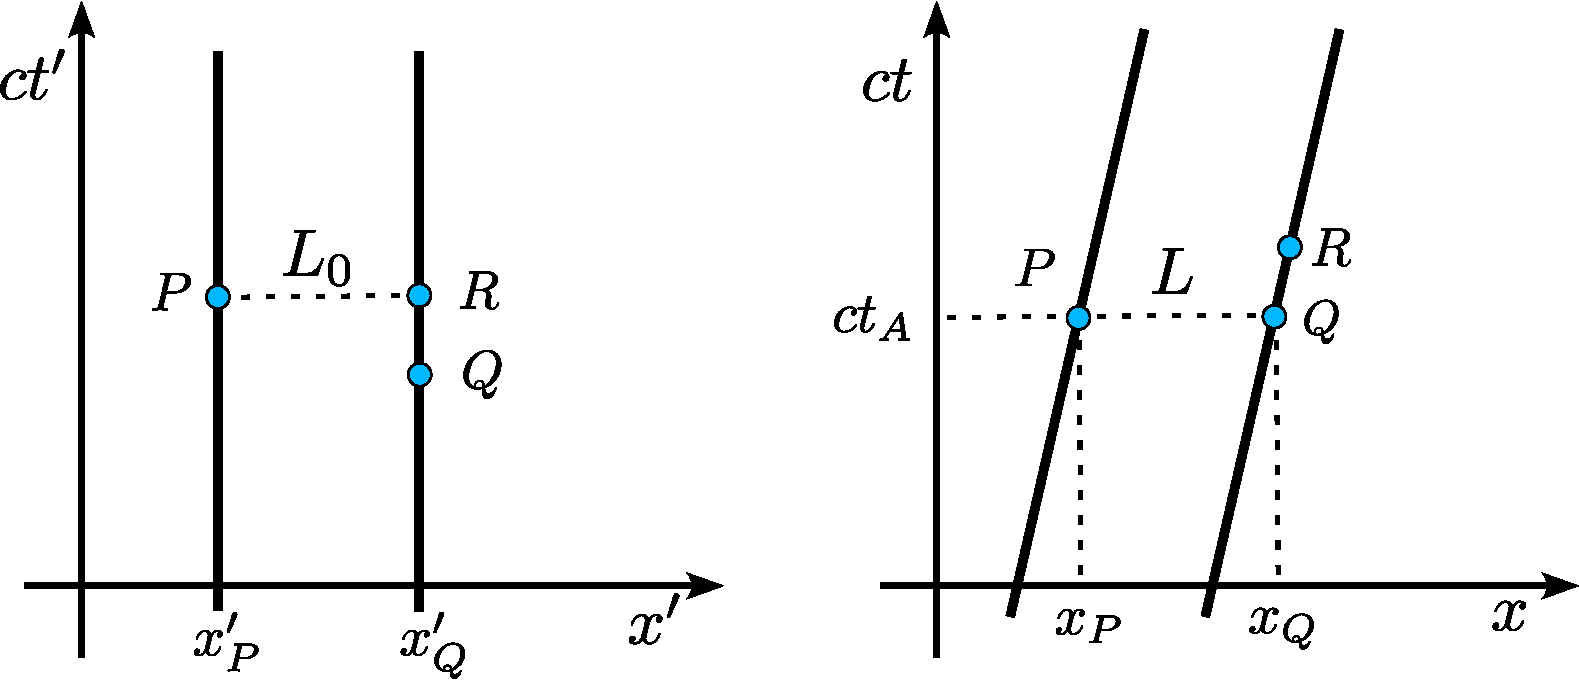
\includegraphics[height= 5cm]{fig/fig-diagrama-contraccion.pdf}}
 \caption{L'ineas de mundo de los extremos de un cuerpo, respecto al SRI com'ovil $K'$ y SRI $K$ donde 'este se mueve con velocidad $v$.}
\label{fcl}
\end{figure}

 Usando la transformaci'on de Lorentz para la posici'on tenemos que el evento $P$ (un extremo del cuerpo) con coordenadas $(ct_A,x_P)$ respecto al SRI $K$ tendr'a, respecto al SRI $K'$ la siguiente posici'on:
\begin{equation}
x'_P=\gamma(x_P-\beta c t_A).
\end{equation}
Por otro lado, el evento $Q$ (en el otro extremo del cuerpo) que es \textit{simult'aneo al evento} $P$ respecto al SRI $K$, tiene coordenadas
\begin{equation}
x'_Q=\gamma(x_Q-\beta c t_A).
\end{equation}
Por lo tanto,
\begin{equation}
x'_Q-x'_P=\gamma(x_Q-x_P),
\end{equation}
En otras palabras, los largos del cuerpo respecto a los dos SRI's est'an relacionados por
\begin{equation}
L=\frac{L_0}{\gamma}<L_0,
\end{equation}
donde $L_0:=x'_Q-x'_P$ es el largo del cuerpo respecto al SRI com'ovil, tambi'en llamado \textit{longitud en reposo} del cuerpo.

Resumiendo, \textbf{todo cuerpo que tiene una longitud $L_0$ respecto a un SRI com'ovil parece tener una longitud \textit{menor} (contracci'on) en un SRI respecto al cual el cuerpo est'a en movimiento}.

\subsection{El cono de luz}
En la teor'ia de la Relatividad, un muy 'util concepto es el \textit{cono de luz}. Por definici'on, el cono de luz asociado a un evento $O$ es el \textit{conjunto de eventos en el espaciotiempo que pueden ser conectados con $O$ por se\~nales luminosas}.
\begin{figure}[!h]
\centerline{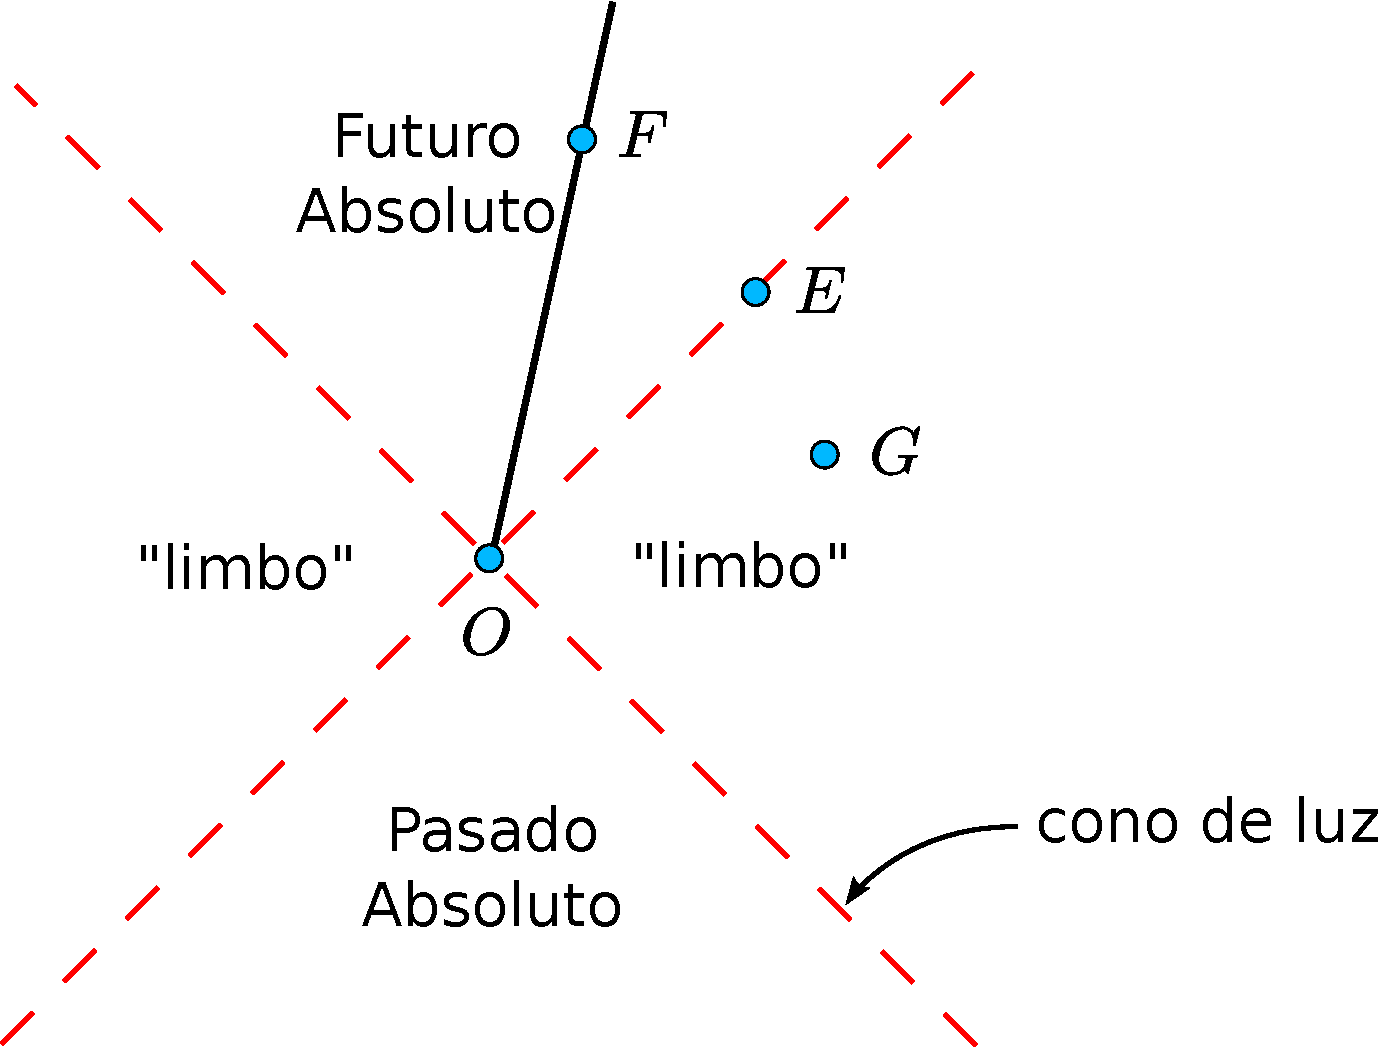
\includegraphics[height= 5cm]{fig/fig-cono-de-luz-1D.pdf}}
 \caption{Cono de luz en 1+1 dimensiones: futuro, pasado absoluto y ``limbo''}
\label{lc}
\end{figure}
El cono de luz divide el espaciotiempo en tres regiones: ``dentro del cono de luz'', ``fuera del cono de luz'' (el ``limbo'') y ``sobre el cono de luz''. Esta clasificaci'on es \textit{absoluta}, en el sentido que no depende del SRI respecto al cual se describan los eventos.

Los eventos \textit{dentro} del cono de luz asociado a $O$ son aquellos que \textit{pueden tener conexi'on causal} con $O$. Es posible adem'as separar los eventos dentro del cono de luz en dos regiones: el \textit{futuro absoluto} y el \textit{pasado absoluto}. Los eventos en el futuro absoluto de $O$ son aquellos que pueden (en principio) ser alcanzados por part'iculas o se\~nales emitidas desde  $O$  y que viajen con velocidades menores que la de la luz. An'alogamente, los eventos en el pasado absoluto de $O$ son aquellos desde los cuales pueden ser emitidas part'iculas o se\~nales viajando con velocidades menores que la de la luz y que pueden eventualmente llegar a $O$. 

Por otro lado, los eventos \textit{fuera} del cono de luz no tienen conexi'on causal con $O$, no pueden afectar a $O$, ni $O$ puede afectar eventos en esa regi'on, ya que eso requerir'ia se\~nales propag'andose con velocidades superluminales.

La clasificaci'on de eventos asociada el cono de luz est'a relacionada con los valores que asume el intervalo entre dos eventos. Si $(t_O,x_O)$ son las coordenadas del evento $O$ y $(t,x)$ las de un evento $P$ cualquiera, entonces podemos calcular $\Delta s^2:=c^2(\Delta t)^2-(\Delta x)^2$. Este valor puede ser positivo, negativo, o nulo.
\begin{itemize}
\item Si $\Delta s^2>0$ entonces el evento $P$ est'a dentro del cono de luz de $O$. Se dice que el vector $OP$ es \textit{tipo tiempo}. Si adem'as $\Delta t>0$ entonces $P$ est'a en el futuro absoluto de $O$, y si $\Delta t<0$, en su pasado absoluto. Los eventos $O$ y $P$ pueden tener conexi'on causal. Es posible encontrar un SRI respecto al cual $O$ y $P$ tienen la misma posici'on espacial, e.d. un SRI com'ovil con estos eventos. No es posible encontrar un SRI respecto al cual $O$ y $P$ sean simult'aneos.

\item Si $\Delta s^2<0$ entonces el evento $P$ est'a fuera del cono de luz de $O$. Se dice que el vector $OP$ es \textit{tipo espacio}. Los eventos $O$ y $P$ no tienen conexi'on causal. Es posible encontrar un SRI respecto al cual $O$ y $P$ son simult'aneos. Tambi'en es posible encontrar SRI's respecto a los cuales $P$ anteceda a $O$, y viceversa. En otras palabras, en este caso $O$ y $P$ no tienen un orden temporal absoluto. No es posible encontrar un SRI respecto al cual $O$ y $P$ tienen la misma posici'on espacial.

\item Si $\Delta s^2=0$ entonces el evento $P$ est'a sobre del cono de luz de $O$. Se dice que el vector $OP$ es \textit{tipo luz}. No es posible encontrar un SRI respecto al cual $O$ y $P$ son  simult'aneos. Tampoco es posible encontrar un SRI respecto al cual $O$ y $P$ tienen la misma posici'on espacial. S'olo se\~nales luminosas (o, en general, part'iculas o se\~nales que se muevan a la velocidad de la luz) pueden conectar $O$ y $P$.
\end{itemize}

\begin{figure}[t]
\centering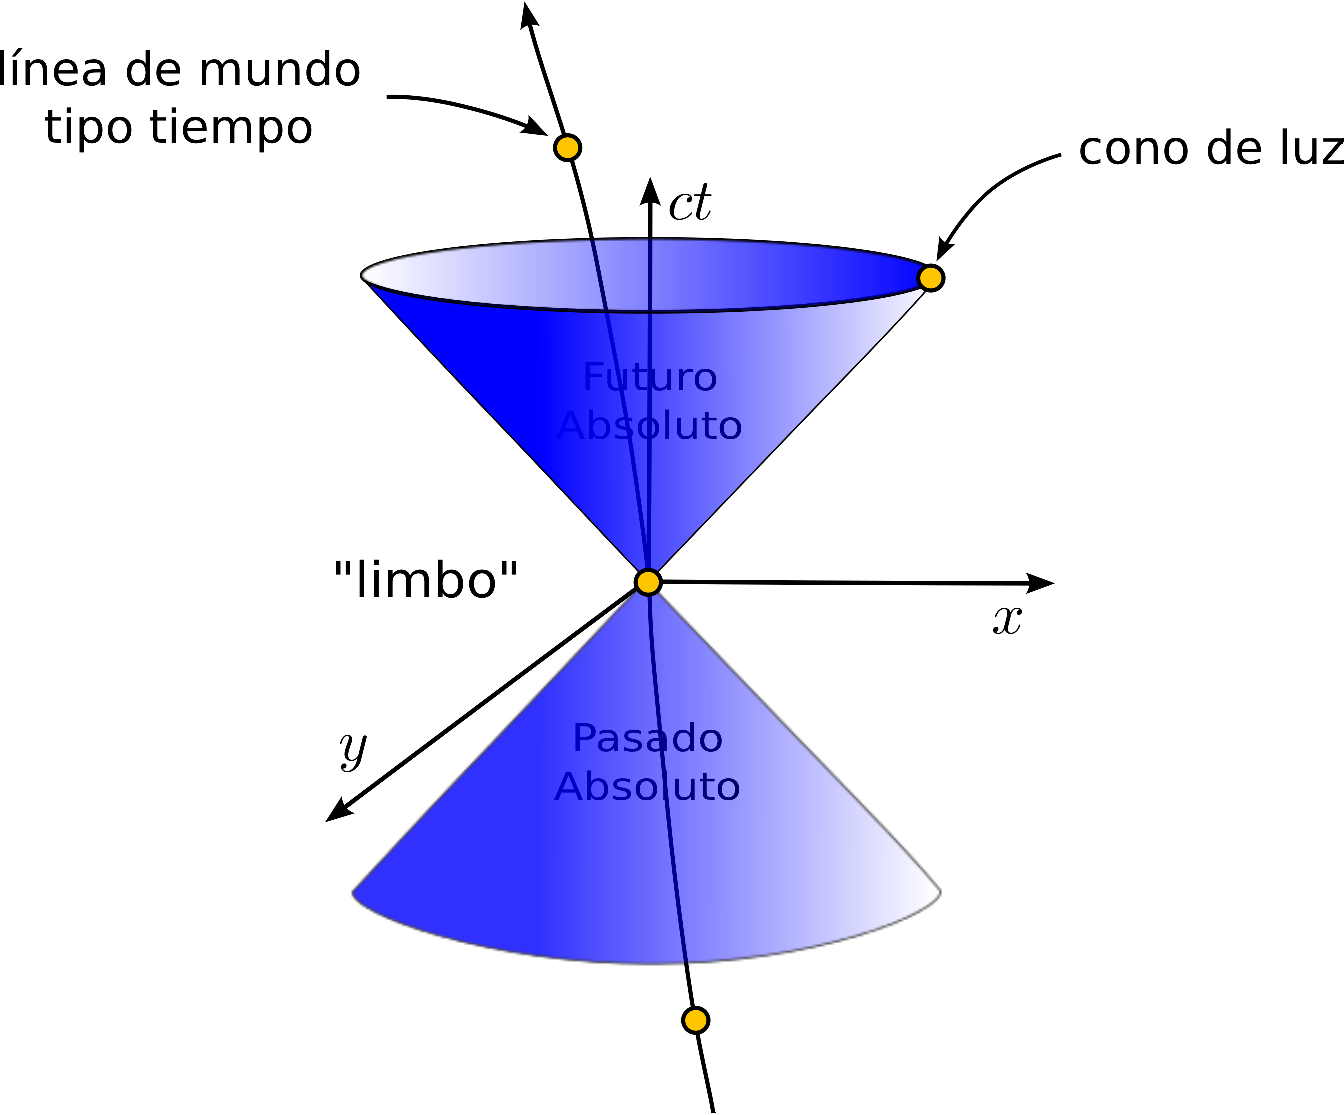
\includegraphics[height=7cm]{fig/fig-cono-de-luz-2D.pdf}
\caption{Cono de Luz, en 2+1 dimensiones.}
\end{figure}



\subsection{Boost en una direcci'on arbitraria}
En la secci'on \ref{secboostx} asumimos impl\'icitamente que las coordenadas asociadas a las direcciones normales ($y$ y $z$) a la velocidad relativa de los dos SRI's (eje $x$) no son alteradas por la transformaci'on (la contracci'on de Lorentz s'olo se produce en la direcci'on de movimiento). En otras palabras, las transformaciones \eqref{boost1} son complementadas con $y'=y$ y $z'=z$. Podemos generalizar este resultado al caso en que la velocidad relativa entre los SRI's $K$ y $K'$ est'a dirigida en una direcci'on arbitraria, separando los vectores $\vec{x}$ y $\vec{x}'$ en componentes paralelas y perpendicular a la velocidad relativa $\vec{V}=c\vec{\beta}$. Usando el hecho que la componente perpendicular es inalterada, y adem'as el boost unidimensional \eqref{boost1} para la componente paralela, es decir, $\vec{x}'_\perp=\vec{x}_\perp$ mientras que  $x'_\parallel=\gamma(x_\parallel-\beta ct)$, con $x_\parallel:=\hat{\beta}\cdot\vec{x}$, $\vec{x}_\perp=\vec{x}-x_\parallel\hat{\beta}$, $\hat{\beta}=\vec{V}/V=\vec{\beta}/\beta$, etc., es simple verificar que la TL correspondiente a un boost en una direcci'on arbitraria es de la forma
\begin{equation}\label{bg1}\marginnote{Boost direcci'on arbitraria}
\boxed{\vec{x}' =\vec{x}+\frac{\left(  \gamma-1\right)  }{\beta^2}\left(  \vec{\beta}\cdot\vec{x}\right)  \vec{\beta}-\gamma ct\vec{\beta},}
\end{equation}
\begin{equation}\label{bg2}
\boxed{ct' = \gamma\left( ct-\vec{\beta}\cdot\vec{x}\right).}
\end{equation}
Esta TL describe el cambio entre los SRI's $K$ y $K'$, tal que $K'$ se mueve con velocidad $\vec{V}=c\vec{\beta}$ respecto a $K$, pero donde los ejes espaciales de $K$ y $K'$ son paralelos (en este sentido, esta TL \textit{no incluye rotaciones}).

\subsubsection{Composici'on de velocidades.}

Considere una part'icula movi'endose con una velocidad
$\vec{v}={d\vec{x}}/{dt}$ en el sistema $K$
\textquestiondown Con qu'e velocidad se mueve la part'icula en el
sistema $K'$, que se mueve con una velocidad $c\vec{\beta}$ con respecto al sistema $K$?.

Considere la TL de un boost general dada por (\ref{bg1})-(\ref{bg2}). En este
caso, para dos eventos infinitesimalmente pr'oximos con coordenadas
$(ct,\vec{x})$ y $(ct+cdt,\vec{x}+d\vec{x})$ respecto a $K$, las diferencias
$d\vec{x}'$ y $dt'$ asociadas a $K'$ est'an dadas por:
\begin{eqnarray}
d\vec{x}'  &  =&d\vec{x}+\frac{\left(  \gamma-1\right)  }{\beta^2}\left(  \vec{\beta}\cdot d\vec{x}\right)  \vec{\beta}-\gamma
c\,dt\vec{\beta},\\
cdt'  &  =&\gamma\left( cdt-\vec{\beta}\cdot d\vec{x}\right)  .
\end{eqnarray}
En el caso en que estos incrementos sean aquellos correspondientes al movimiento
de una part'icula, velocidad es dada por
$\vec{v}:={d\vec{x}}/{dt}$ respecto a $K$ y
$\vec{v}':={d\vec{x}'}/{dt'}$ respecto a $K'$. Por lo tanto, encontramos que
\begin{equation}
\frac{1}{c}\vec{v}'=\frac{1}{c}\frac{d\vec{x}'}{dt'}=\frac{\frac{d\vec{x}}{dt}
+\frac{\left(  \gamma-1\right)  }{\beta^2}\left(  \vec{\beta}\cdot
\frac{d\vec{x}}{dt}\right)  \vec{\beta}-\gamma c\vec{\beta}}{\gamma\left(
c-\vec{\beta}\cdot \frac{d\vec{x}}{dt}\right) },
\end{equation}
es decir,
\begin{equation}
\boxed{
\vec{v}'=\frac{\vec{v}+\frac{\left(  \gamma-1\right)  }{\beta^2}\left(
\vec{\beta}\cdot \vec{v}\right)  \vec{\beta}-\gamma c\vec{\beta}}{\gamma\left(
1-\vec{\beta}\cdot \frac{\vec{v}}{c}\right) }.
} \label{transv}
\end{equation}
Equivalentemente,
\begin{equation}
\vec{v}'_\parallel=\frac{\vec{v}_\parallel- c\vec{\beta}}{1-\vec{\beta}\cdot\frac{\vec{v}_\parallel}{c} }, \qquad 
\vec{v}'_\perp=\frac{\vec{v}_\perp}{\gamma\left(
1-\vec{\beta}\cdot \frac{\vec{v}_\parallel}{c}\right) }
\end{equation}
donde hemos definido la velocidad paralela y perpendicular (respecto a $\vec\beta$), $\vec{v}_\parallel:=(\vec{v}\cdot \hat\beta)\hat\beta$,  $\vec{v}_\perp:=\vec{v}-\vec{v}_\parallel$.

\subsection{Incompatibilidad de las definiciones newtonianas de energ'ia y momentum lineal con el Principio de Relatividad}

En mec'anica no-relativista se define el momentum lineal de una part'icula como
$\vec{p}:=m\vec{v}$, donde $\vec{v}$ es la velocidad de la part'icula (que
depende del SRI), y $m$ es la masa de la part'icula (que \textit{no depende} del SRI, es un escalar). La caracter'istica principal del momentum es su propiedad de conservaci'on en un sistema aislado (por ejemplo, en un choque de part'iculas). Adem'as, la \textit{ley de conservaci'on del momentum lineal} es v'alida (para un sistema aislado de part'iculas) \textit{en todo SRI}. Es simple verificar, usando la ley newtoniana (o``Galileana'') de  transformaci'on de la velocidad de un cuerpo entre SRI's, que si el momentum de un sistema de part'iculas es conservado en un SRI entonces ser'a conservado en todo SRI. 

Sin embargo, usando las leyes \textit{relativistas} de transformaci'on de la velocidad, ec. \eqref{transv}, y asumiendo que el momentum sigue siendo $\vec{p}:=m\vec{v}$ y que $m$ es un escalar, entonces puede comprobarse que la ley de conservaci'on del momentum de un sistema de part'iculas \textit{no ser'a v'alida (``simult'aneamente'') en todo SRI} (es decir, no respetar'a el Principio de Relatividad). Por ejemplo en un choque de dos part'iculas, si en un SRI particular $K$ se verifica que $m_1\vec{v}_{1i}+m_2\vec{v}_{2i} =m_1\vec{v}_{1f}+m_2\vec{v}_{2f}$, entonces, \eqref{transv} implican en general que, $m_1\vec{v}'_{1i}+m_2\vec{v}'_{2i} \neq m_1\vec{v}'_{1f}+m_2\vec{v}'_{2f}$ en otros SRI's $K'$.

Considere el siguiente caso simple de una colisi'on de part'iculas id'enticas, todas de masa $m$.
Las velocidades iniciales y finales de las part'iculas $1$ y $2$ est'an dadas, respecto al SRI $K$ (del centro de masa), por
\begin{equation}
 \vec{v}_{1i}=v \hat{x}, \qquad \vec{v}_{2i}=-v \hat{x},
\end{equation}
\begin{equation}
 \vec{v}_{1f}=v \hat{y}, \qquad \vec{v}_{2f}=-v \hat{y}.
\end{equation}
Ahora realizamos un boost con velocidad relativa $c\vec\beta=v\hat{x}$, hasta el SRI $K'$ com'ovil con la part'icula 1 en su movimiento inicial (SRI ``de laboratorio''). Utilizando la ley de transformaci'on relativista de velocidades (\ref{transv}), obtenemos las velocidades respecto al nuevo SRI:
\begin{equation}
 \vec{v}'_{1i}=\vec{0}, \qquad \vec{v}'_{2i}=-\frac{2v \hat{x}}{1+v^2/c^2},
\end{equation}
\begin{equation}
 \vec{v}'_{1f}=-v\hat{x}+\frac{v}{\gamma} \hat{y}, \qquad \vec{v}'_{2f}=-v\hat{x}-\frac{v}{\gamma} \hat{y}.
\end{equation}
Si el momentum de cada part'icula es de la forma $\vec{p}=m\vec{v}$ entonces, el momentum total en el SRI de centro de masa es dado por
\begin{equation}
 \vec{p}_i=\vec{p}_{1i}+\vec{p}_{2i}=\vec{0},
\end{equation}
\begin{equation}
 \vec{p}_f=\vec{p}_{1f}+\vec{p}_{2f}=\vec{0},
\end{equation}
es decir, se conserva el momentum lineal total. Sin embargo, en el SRI de laboratorio tendremos que
\begin{equation}
 \vec{p}'_i=\vec{p}'_{1i}+\vec{p}'_{2i}=-\frac{2mv\hat{x}}{1+v^2/c^2},
\end{equation}
mientras que
\begin{equation}
 \vec{p}'_f=\vec{p}'_{1f}+\vec{p}'_{2f}=-2mv\hat{x}.
\end{equation}

Similarmente, puede verificarse que lo mismo ocurre con la energ'ia. 
Si asumimos que la energ'ia (cin'etica) de una part'icula de masa $m$ y velocidad $\vec{v}$ es dada por la usual expresi'on norelativista, entonces en el SRI del centro de masa la energ'ia se conserva en el proceso analizado:
\begin{equation}
 E_i=\frac{1}{2}m\vec{v}_{1i}^2+\frac{1}{2}m\vec{v}_{2i}^2=mv^2,
\end{equation}
\begin{equation}
 E_f=\frac{1}{2}m\vec{v}_{1f}^2+\frac{1}{2}m\vec{v}_{2f}^2=mv^2.
\end{equation}
Sin embargo, en el SRI de laboratorio
\begin{equation}
 E'_i=\frac{1}{2}m\vec{v}'_{1i}{}^2+\frac{1}{2}m\vec{v}'_{2i}{}^2=\frac{2mv^2}{(1+v^2/c^2)^2},
\end{equation}
mientras que
\begin{equation}
 E'_f=\frac{1}{2}m\vec{v}'_{1f}{}^2+\frac{1}{2}m\vec{v}'_{2f}{}^2=mv^2\left(2-v^2/c^2\right).
\end{equation}
Claramente, en general (es decir, para valores arbitrarios de $v$),  $ E'_i\neq E'_f$. ! Este resultado se contradice con el esperado a partir del Principio de Relatividad: que si la energ'ia se conserva en un SRI, entonces debe conservarse en todo SRI. Si esto no fuese as'i, entonces existir'ian SRI's ``privilegiados'' o ``especiales'': aquel SRI donde s'i se conserva la energ'ia en un choque. El mismo argumeto es aplicable al momentum lineal.

En resumen, \textit{en RE la definici'on newtoniana de la energ'ia y el momentum de un cuerpo es incompatible con el Prinicpio de Relatividad}, es decir, con la equivalencia entre SRI's. Por esto, es necesario reemplazar las definiciones newtonianas por unas que s'i respeten este principio, es decir, que satisfagan el requerimiento que si la energ'ia es conservada en un SRI, entonces sea conservada \textit{en todo SRI}, y similarmente para el momentum.

Como veremos m'as adelante, en la teor'ia de RE se reemplazan las definiciones newtonianas de energ'ia y momentum lineal por nuevas definiciones (en t'erminos de la masa y velocidad del cuerpo) que s'i son compatibles en el Principio de Relatividad. Las \textit{expresiones relativistas de energ'ia y momentum} son
\begin{equation}
E=\frac{mc^2}{\sqrt{1-\frac{v^2}{c^2}}}, \qquad \vec{p}=\frac{m\vec{v}}{\sqrt{1-\frac{v^2}{c^2}}}.
\end{equation}

Para \textit{probar} que estas nuevas definiciones realmente satisfacen las propiedades requeridas, es de mucha utilidad expresar estas cantidades en t'erminos de vectores y tensores \textit{respecto a Transformaciones de Lorentz} (que relacionan SRI's): los llamados 4-vectores y 4-tensores (``cuadri-vectores'' y ``cuadri-tensores''). Por esto, a continuaci'on revisaremos r'apidamente la definici'on y propiedades b'asicas de estos objetos.


\section{La visi'on Cuadridimensional}
En la teor'ia newtoniana el tiempo es absoluto, de modo que el espaciotiempo (es decir, el conjunto de todos los eventos) se separa naturalmente en espacio + tiempo. Matem'aticamente, esto significa que
bajo las transformaciones m'as generales que relacionan un SRI con otro
(Transformaciones de Galileo, Rotaciones y translaciones) tanto los intervalos de
tiempo entre eventos (infinitesimalmente pr'oximos), con coordenadas
$(t,\vec{x})$ y $(t+dt,\vec{x}+d\vec{x})$ respecto a un SRI, como la
distancia entre ellos permanecen invariantes, es decir,
\begin{equation}
dt'=dt, \qquad d\vec{x}^2=d\vec{x}'^2.
\end{equation}
La condici'on de invariancia de $d\vec{x}^2$, permite asociar un concepto
absoluto de distancia: \textit{una geometr'ia tridimensional euclideana}, donde las coordenadas de un evento respecto a un SRI son relativas (cambian bajo transformaci'on de SRI), pero la distancia $d\vec{x}^2$ es absoluta.

Por otro lado, en la teor'ia especial de la relatividad, la distancia espacial $d\vec{x}^2$ no es absoluta, como tampoco lo es $dt$ (``los boosts mezclan espacio y tiempo''). Sin embargo, el as'i llamado \textit{intervalo},
\begin{equation}
ds^2:=c^2dt^2-d\vec{x}^2, \label{ds}
\end{equation}
es invariante bajo transformaciones entre SRI's. En este sentido, \textit{el
intervalo es una magnitud absoluta en RE}. En analog'ia al caso newtoniano, esto permite introducir una geometr'ia, interpretando $ds^2$ como una especie de ``distancia'' en el espaciotiempo 4-dimensional: el \textit{espacio de Minkowski}\footnote{Hermann Minkowski (1864-1909): matem'atico alem'an. Ver \url{http://es.wikipedia.org/wiki/Hermann_Minkowski}.} (1907, ver \cite{Minkowski07}).

\begin{center}
\boxed{
\parbox{12cm}{$ds^2:=c^2dt^2-d\vec{x}^2$ define la geometr'ia (pseudo-)euclideana del espaciotiempo de Minkowski.}}
\end{center}
Por ejemplo, el boost en la direcci'on $x$ puede ser expresado en t'erminos de una matriz de transformaci'on:
\begin{equation}
 \left(\begin{array}{c} ct' \\ x' \\ y' \\z' \end{array}\right)=\left(
\begin{array}{cccc}
\gamma & -\gamma\beta & 0 &0 \\
-\gamma\beta & \gamma  & 0  & 0 \\
0 & 0 & 1  & 0 \\
0 & 0 & 0  & 1
\end{array}
\right)\left(\begin{array}{c} ct \\ x \\ y \\z \end{array}\right).
\end{equation}

Ahora estamos en condiciones de definir m'as generalmente una Transformaci'on de Lorentz. 

\begin{quotation}
\boxed{
\parbox{12cm}{Las \textit{transformaciones de Lorentz} (TL's) son definidas como aquellas transformaciones lineales de las (4) coordenadas de un evento, entre 2 SRI's, y que dejan el intervalo $ds^2$ \textit{invariante}, es decir, tales que $c^2dt^2-d\vec{x}^2=c^2dt'^2-d\vec{x}'^2$.}}
\end{quotation}


Con esta definici'on, las TL's incluyen los boost's (TL's simples) en una direcci'on arbitraria, las rotaciones, reflexiones espaciales y temporales (estos tres 'ultimos tipos de transformaci'on dejan $dt^2$ y $d\vec{x}^2$ separadamente invariantes), \textit{y sus composiciones}. Matem'aticamente, el conjunto de todas las TL's forma un \textit{grupo}: el grupo de Lorentz.

Recuerde que la interpretaci'on f'isica de $ds$ es que, para eventos con separaci'on tipo tiempo ($ds^2>0$) la cantidad $d\tau=ds/c$ es el \textit{tiempo propio entre dos eventos} (infinitesimalmente pr'oximos), es decir el tiempo registrado por un observador com'ovil con los eventos. Esto puede verificarse en el SRI en el que los dos eventos aparezcan en el mismo punto del espacio, es decir, $d\vec{x}^2=0$, ya que en este caso $ds=c\,dt$.
\subsection{4-vectores y 4-tensores}

Denotamos las coordenadas de un evento en el espaciotiempo,
respecto de un SRI $K$, colectivamente por $x^\mu$, con $\mu=0,1,2,3$, de modo que $x^0:=ct$, $x^1:=x$, $x^2:=y$, $x^3:=z$. En general, los 'indices griegos $\mu,\nu,\lambda,\cdots$ variar'an de 0 a 3, mientras que los latinos
$i,j,k,\cdots$ lo har'an de 1 a 3. As'i, por ejemplo, denotaremos
$x^\mu=(x^0,x^i)$ o, equivalentemente, $x^\mu=(x^0,\vec{x})$.

Bajo una TL, las coordenadas de un evento cambiar'an, por ejemplo de $x^\mu$ a
$x'^\mu$ cuando cambiemos de un SRI $K$ a otro $K'$. La TL m'as general, que
incluye boosts, ver (\ref{boost1}), y rotaciones, es lineal en las coordenadas
espaciotemporales y por tanto puede escribirse en la forma
\begin{equation}\label{xpLx}
x'^\mu=\Lambda^\mu_{\ \nu}x^\nu ,
\end{equation}
donde $\Lambda^\mu_{\ \nu}$ son, para cada transformaci'on, 16 constantes. Adem'as, las componentes $\Lambda^\mu_{\ \nu}$ deben ser tales que el intervalo permanezca invariante: $ds'^2=ds^2$.
En (\ref{xpLx}) hemos usado la convenci'on de suma de Einstein, de suma de
'indices repetidos, de modo que $\Lambda^\mu_{\
\nu}x^\nu:=\Lambda^\mu_{\ 0}x^0+ \Lambda^\mu_{\ 1}x^1+ \Lambda^\mu_{\ 2}x^2+\Lambda^\mu_{\ 3}x^3$.

Por ejemplo, la matriz $\Lambda^\mu_{\ \nu}$ correspondiente al boost (\ref{bg1})-(\ref{bg2}) es dada por:
\begin{equation}
\Lambda^\mu_{\ \nu}=\left(
\begin{array}
[c]{cccc}
\gamma & -\gamma\beta^x & -\gamma\beta^y & -\gamma\beta^z\\
-\gamma\beta^x & 1+\frac{(\beta^x)^2}{\beta^2}\left(\gamma-1\right)  &
\frac{\beta^x\beta^y}{\beta^2}\left(\gamma-1\right)  & \frac{\beta^x\beta^z}{\beta^2}\left(\gamma-1\right) \\
-\gamma\beta^y & \frac{\beta^y\beta^x}{\beta^2}\left(\gamma-1\right)
& 1+\frac{(\beta^y)^2}{\beta^2}\left(\gamma-1\right)  & \frac{\beta
^y\beta^z}{\beta^2}\left(  \gamma-1\right) \\
-\gamma\beta^z & \frac{\beta^z\beta^x}{\beta^2}\left(\gamma-1\right)
& \frac{\beta^z\beta^y}{\beta^2}\left(\gamma-1\right)  & 1+\frac{(\beta^z)^2}{\beta^2}\left(\gamma-1\right)
\end{array}
\right), \label{boostgen}
\end{equation}
con $\vec\beta=(\beta^x,\beta^y,\beta^z)$ y $\beta^2=(\beta^x)^2+(\beta^y)^2+(\beta^z)^2$.

Por otro lado, una \textit{rotaci'on general} es de la forma
\begin{equation}
\Lambda^\mu_{\ \nu}=\left(
\begin{array}[c]{c|c}
1 & 0_3 \\
\hline
0_3 & \mathbf{R}
\end{array}
\right), \label{rotgen}
\end{equation}
donde $\mathbf{R}$ es una matriz \textit{ortogonal} de $3\times 3$, es decir, que satisface $\mathbf{R}\mathbf{R}^\top=\mathbf{1}_{3\times 3}$. Esta transformaci'on preserva $dt^2$ y $d\vec{x}^2$ \textit{por separado}.

Tal como en mec'anica newtoniana es 'util expresar las leyes f'isicas usando
vectores y tensores respecto a rotaciones, en RE es conveniente (pero no
obligatorio!) usar vectores, tensores, etc., definidos \textit{con respecto  a TL's}.

\subsubsection{Escalares (\textit{invariantes})}
Un escalar es una cantidad que \textit{no cambia su valor bajo TL's}. Si $\phi(P)$ es una cantidad asociada al evento $P$ respecto al SRI $K$, y $\phi'(P)$ es la misma cantidad, asociada al mismo evento, pero con respecto a otro SRI arbitrario $K'$, entonces $\phi(P)$ es un escalar si y s'olo si
\begin{equation}
\phi'(P)=\phi(P).
\end{equation}
Ejemplos de cantidades escalares bajo TL's: las masas y las cargas de
las part'iculas, la rapidez de la luz, el intervalo.

\subsubsection{4-vector \textit{contravariante}}
Se dice que conjunto de 4 cantidades, $A^\mu$ ($\mu=0,1,2,3$), definidas en cada SRI (y denotadas, por convenci'on, usando un \textit{super'indice}), son las componentes de un 4-vector contravariante si sus valores respecto a dos SRI's relacionados por una TL arbitraria, est'an relacionadas tal como las coordenadas espaciotemporales, es decir, por
\begin{equation}
A'^\mu=\Lambda^\mu_{\ \nu} A^\nu .
\end{equation}
Ejemplos: 4-posici'on, 4-velocidad, 4-momentum.

\subsubsection{4-vector \textit{covariante}}
Se dice que un conjunto de 4 cantidades, $A_\mu$ ($\mu=0,1,2,3$), definidas en cada SRI (y denotadas, por convenci'on, usando un \textit{sub'indice}), son las componentes de un 4-vector covariante si sus valores respecto a dos SRI's relacionados por una TL arbitraria, est'an relacionadas por
\begin{equation}
A'_\mu=\left( \Lambda^{-1}\right)^\nu _{\ \mu}A_{\nu},
\end{equation}
donde $\left( \Lambda^{-1}\right)^\nu _{\ \mu}$ es la TL \textit{inversa}, definida de modo que
\begin{equation}
\Lambda^\mu_{\ \lambda}\left( \Lambda^{-1}\right)^{\lambda}_{\
\nu}=\delta^\mu_\nu ,
\end{equation}
y donde $\delta^\mu_\nu$ es la delta de Kronecker, definida en todo SRI por 
$\delta^0_0=\delta^1_1=\delta^2_2=\delta^3_3=1$, y $\delta^\mu_\nu=0$ si
$\mu\neq\nu$. 

Ejemplo de vector covariante: el 4-\textit{gradiente} de un campo escalar, $A_\mu:={\partial\phi}/{\partial x^\mu}=\partial_\mu\phi$.

\subsubsection{Tensor de rango $(^p_q)$:}
Un conjunto de $4^{p+q}$ cantidades ($T^{\mu_1 \cdots\mu_p}_{\ \ \ \ \ \ \ \
\nu_1\cdots\nu_q}$) definidas en cada SRI se consideran componentes de un (4-)tensor de rango $(^p_q)$, si sus valores se relacionan, bajo TL's, por
\begin{equation}
T'^{\mu_1 \cdots\mu_p}_{\ \ \ \ \ \ \ \
\nu_1\cdots\nu_q}={\Lambda^{\mu_1}}_{\lambda_1} \cdots
{\Lambda^{\mu_p}}_{\lambda_p} \left( \Lambda^{-1}\right) ^{\rho_1}_{\
\nu_1}\cdots\left( \Lambda^{-1}\right) ^{\rho_q}_{\ \nu_q} T^{\lambda_1
\cdots\lambda_p}_{\ \ \ \ \ \ \ \rho_1\cdots\rho_q}. 
\end{equation}

\subsubsection{Multiplicaci'on de 4-tensores}
 Si $A^{\mu_1 \cdots\mu_p}_{\ \ \ \ \ \ \ \
\nu_1\cdots\nu_q}$ y $B^{\mu_1 \cdots\mu_r}_{\ \ \ \ \ \ \ \
\nu_1\cdots\nu_s}$ son (las $4^{p+q}$ y $4^{r+s}$ componentes de) dos tensores de rango $(^p_q)$ y $(^r_s)$ respectivamente, entonces el
conjunto de $4^{p+q+r+s}$ cantidades definidas por
\begin{equation}
C^{\mu_1 \cdots\mu_{p+r}}_{\ \ \ \ \ \ \ \ \ \
\nu_1\cdots\nu_{q+s}}:=A^{\mu_1 \cdots\mu_p}_{\ \ \ \ \ \ \ \
\nu_1\cdots\nu_q}\times B^{\mu_{p+1} \cdots\mu_{p+r}}_{\ \ \ \ \ \ \ \ \ \ \ \ \, \nu_{q+1}\cdots\nu_{q+s}}
\end{equation}
definen un tensor de rango $(^{p+r}_{q+s})$ bajo TL's.

\subsubsection{Contracci'on de 4-tensores}
 Si $A^{\mu_1 \cdots\mu_p}_{\ \ \ \ \ \ \ \
\nu_1\cdots\nu_q}$ son las $4^{p+q}$ componentes de un tensor de rango $(^p_q)$, entonces las $4^{p+q-2}$ cantidades definidas por la ``contracci'on''
\begin{equation}
B^{\mu_1 \cdots\mu_{n-1}\mu_{n+1}\cdots\mu_p}_{\ \ \ \ \ \ \ \ \ \ \ \ \ \ \ \ \ \ \ \ \nu_1\cdots\nu_{m-1}\nu_{m+1}\cdots\nu_q}:=A^{\mu_1
\cdots\mu_{n-1}\rho\mu_{n+1}\cdots\mu_p}_{\ \ \ \ \ \ \ \ \ \ \ \ \ \ \ \ \ \ \
\ \ \nu_1\cdots\nu_{m-1}\rho\nu_{m+1}\cdots\nu_q},
\end{equation}
son componentes de un tersor de rango $(^{p-1}_{q-1})$.

\paragraph{Observaciones:}

\begin{itemize}
\item Un escalar es un tensor de rango $(^0_0)$.
\item Un vector contravariante es un tensor de rango $(^1_0)$.
\item Un vector covariante es un tensor de rango $(^0_1)$.
\item La delta de Kronecker define un \textit{tensor invariante} de rango $(^1_1)$ bajo TL's, es decir, que sus componentes tienen el mismo valor en todo SRI.
\item Podemos definir adem'as el \textit{s'imbolo de Levi-Civita contravariante} $\hat\epsilon^{\mu\nu\lambda\rho}$ como el \textit{(pseudo-)tensor invariante} bajo TL's que es totalmente antisim'etrico y que satisface $\hat\epsilon^{0123}:=1$.
\item An'alogamente, podemos definir el \textit{s'imbolo de Levi-Civita
covariante} $\epsilon_{\mu\nu\lambda\rho}$ como el \textit{(pseudo-)tensor invariante} bajo TL's (de determinante 1) que es totalmente antisim'etrico y
que satisface $\epsilon_{0123}:=1$.

\item La utilidad de los tensores, reside en el hecho que las relaciones que
involucran tensores del mismo grado, son ecuaciones 
\textit{invariantes de forma}\footnote{Tambi'en llamadas, abusando un poco del lenguaje, ecuaciones \textit{covariantes}.} bajo TL's, esto es, si
\begin{equation}
T^{\mu_1 \mu_2 ... \mu_r}=0,
\end{equation}
entonces en todo otro SRI 
\begin{equation}
T'^{\nu_1 \nu_2 ... \nu_r}=0.
\end{equation}
Como las TL's expresan matem'aticamente el cambio desde un SRI a otro, entonces \textbf{una forma de garantizar autom'aticamente que una cierta ley f'isica respeta la equivalencia entre SRI's, es decir, el Principio de Relatividad, es expresando dicha ley en funci'on de cantidades que sean tensores bajo TL's}. Esto es an'alogo al caso newtoniano, donde el hecho de escribir las leyes de la F'isica en t'erminos de vectores y tensores tridimensionales (por ejemplo,
$\vec{F}=m\vec{a}$, o bien $D_i=\varepsilon_{ij}E_j$), que transforman homog'eneamente (como vectores y tensores) bajo \textit{rotaciones}, asegura que esta ley tendr'a \textit{la misma forma} en cualquier sistema de coordenadas cartesiano, independiente de la orientaci'on espacial de sus ejes. En otras palabras, el uso de vectores y tensores tridimensionales para expresar las leyes f'isicas resulta conveniente puesto que incorpora naturalmente la equivalencia de sistemas de coordenadas cartesianos respecto a rotaciones. Del mismo modo, el expresar una ley f'isica en t'erminos de 4-tensores bajo TL's asegura que esta ley respeta el Principio de Relatividad de RE.

\end{itemize}

\subsubsection{Identidades}

\paragraph{Antisimetrizaci'on:}

\begin{equation}
T_{[\mu\nu]}:=\frac{1}{2}(T_{\mu\nu}-T_{\nu\mu}),
\end{equation}
\begin{equation}
T_{[\mu\nu\lambda]}:=\frac{1}{3}(T_{\mu[\nu\lambda]}+T_{\nu[\lambda\mu]}+T_{
\lambda[\mu\nu]}),
\end{equation}
\begin{equation}
T_{[\mu\nu\lambda\rho]}:=\frac{1}{4}(T_{\mu[\nu\lambda\rho]}-T_{\nu[
\lambda\rho\mu]}+T_{\lambda[\rho\mu\nu]}-T_{\rho[\mu\nu\lambda]})\equiv T_{[0123]}\,\epsilon_{\mu\nu\lambda\rho}.
\end{equation}

\paragraph{Propiedades de los s'imbolos de Levi-Civita:}
\begin{eqnarray}
\hat\epsilon^{\mu\nu\lambda\rho}\, \epsilon_{\alpha\beta\gamma\delta}
&\equiv& 4!\,\delta^\mu_{[\alpha}\delta ^\nu_\beta \delta^\lambda_\gamma
\delta^\rho_{\delta]}, \\
\hat\epsilon^{\mu\nu\lambda\rho}\, \epsilon_{\alpha\beta\gamma\rho}
&\equiv& 3!\,\delta^\mu_{[\alpha}\delta ^\nu_\beta \delta^\lambda_{\gamma]}, \\
\hat\epsilon^{\mu\nu\lambda\rho}\, \epsilon_{\alpha\beta\lambda\rho}
&\equiv& 2! \left(\delta^\mu_\alpha\delta ^\nu_\beta -  \delta^\nu_\alpha \delta^\mu_\beta \right),\\
\hat\epsilon^{\mu\nu\lambda\rho}\, \epsilon_{\alpha\nu\lambda\rho}
&\equiv& 3!\,\delta^\mu_\alpha,\\
\hat\epsilon^{\mu\nu\lambda\rho}\, \epsilon_{\mu\nu\lambda\rho}&\equiv& 4!.
\end{eqnarray}


\subsection{M'etrica de Minkowski}
Podemos expresar el escalar $ds$ en t'erminos de 4-tensores. Para esto, notamos
que el 4-desplazamiento $dx^\mu$ es un 4-vector (bajo TL's), de modo que
$dx^\mu dx^\nu$ es un tensor de rango $(^2_0)$. Podemos entonces escribir
el escalar $ds$ en t'erminos de $dx^\mu dx^\nu$ y un nuevo \textit{tensor
m'etrico} de rango $(^0_2)$, que denotaremos por $\eta_{\mu\nu}$, de modo que
\begin{equation}
ds^2:=\eta_{\mu\nu}dx^\mu dx^\nu. \label{dstens}
\end{equation}
Comparando (\ref{dstens}) con (\ref{ds}) encontramos que (en un SRI)
debemos tener que
\begin{equation}
\eta_{00}=-\eta_{11}=-\eta_{22}=-\eta_{33}=1, \qquad \eta_{\mu\nu}=0
\quad\rm{si}\quad \mu\neq\nu .
\end{equation}
Sin embargo, en RE el intervalo $ds$ no es cualquier escalar, sino que tiene el mismo valor en todo SRI \textit{cuando se lo calcula de la misma forma}, tal como en la definici'on (\ref{ds}). Esto significa que, en RE, el tensor m'etrico (o simplemente ``la m'etrica'') $\eta$ debe tener los mismos valores, en cada una de sus componentes, en todo SRI. En  otras palabras, $\eta$ debe ser un tensor \textit{invariante} de rango $(^0_2)$ bajo TL's. Esto significa que
\begin{equation}
\eta'_{\mu\nu}=\left( \Lambda^{-1}\right)^{\lambda}_{\ \mu}\left(
\Lambda^{-1}\right)^{\rho}_{\ \nu}\eta_{\lambda\rho}=\eta_{\mu\nu},
\end{equation}
o, equivalentemente
\begin{equation}
\boxed{\Lambda^\lambda_{\ \mu}\Lambda^\rho_{\ \nu}\eta_{\lambda\rho}=\eta_{\mu\nu}.}
\label{condLor}
\end{equation}
De hecho, es posible considerar (\ref{condLor}) como la condici'on general que define una TL $\Lambda$.

Teniendo el tensor m'etrico a nuestra disposici'on es posible definir el \textit{tensor m'etrico inverso} $\eta^{\mu\nu}$, de rango $(^2_0)$, de modo que
\begin{equation}
\boxed{\eta^{\mu\nu}\eta_{\nu\lambda}=\delta^\mu_\lambda .}\label{definv}
\end{equation}

En notaci'on matricial $\eta^{\mu\nu}$ corresponde a la matriz inversa a la
m'etrica $\eta_{\mu\nu}$. M'as a'un, las componentes de la m'etrica (de
Minkowski) inversa coinciden con aquellas de $\eta_{\mu\nu}$
\begin{equation}
\eta^{00}=-\eta^{11}=-\eta^{22}=-\eta^{33}=1, \qquad \eta^{\mu\nu}=0
\quad\rm{si}\quad \mu\neq\nu .
\end{equation}

El tensor m'etrico $\eta_{\mu\nu}$ permite \textit{asociar} a cada vector
\textit{contravariante} $A^\mu$ un nuevo vector \textit{covariante}  (abusando
un poco de la notaci'on) $A_\mu$, definido por
\begin{equation}
A_\mu:=\eta_{\mu\nu}A^\nu.
\end{equation}
Similarmente, la m'etrica inversa $\eta^{\mu\nu}$ permite asociar un vector
\textit{contravariante} $A^\mu$ a cada vector \textit{covariante} $A_\mu$, por
medio de
\begin{equation}
A^\mu:=\eta^{\mu\nu}A_\nu.
\end{equation}
A partir de (\ref{definv}) es simple verificar que la secuencia de operaciones consistente en tomar un vector contravariante cualquiera, definir su vector covariante asociado, y a partir de este 'ultimo calcular el vector contravariante correspondiente, retorna al vector contravariante original. Lo mismo ocurre si partimos de un vector covariante. Esta propiedad justifica (parcialmente) la convenci'on de uso de la misma letra para un vector covariante y su vector contravariante asociado.

% \subsubsection{Notaci'on Matricial}
%
% Usaremos la convenci'on de que el 'indice superior (contravariante)
% representa las filas, y el inferior (covariante) las columnas de la matriz.
% Por ejemplo, las siguientes expresiones se muestran en notaci'on vectorial
% y tensorial:
% \begin{align}
% x^{\alpha} &  =\Lambda_{\ \beta}^{\alpha}y^{\beta}\Leftrightarrow\left(
% \begin{array}
% [c]{c}%
% x^1\\
% x^2\\
% x^3\\
% x^4%
% \end{array}
% \right)  =\left(
% \begin{array}
% [c]{cccc}%
% \Lambda_1^1 & \Lambda_2^1 & \Lambda_3^1 & \Lambda_{4}^1\\
% \Lambda_1^2 & \Lambda_2^2 & \Lambda_3^2 & \Lambda_{4}^2\\
% \Lambda_1^3 & \Lambda_2^3 & \Lambda_3^3 & \Lambda_{4}^3\\
% \Lambda_1^4 & \Lambda_2^4 & \Lambda_3^4 & \Lambda_{4}^4%
% \end{array}
% \right)  \left(
% \begin{array}
% [c]{c}%
% y^1\\
% y^2\\
% y^3\\
% y^4%
% \end{array}
% \right)  \\
% x_{\beta} &  =y_{\alpha}\Omega_{\ \beta}^{\alpha}\Leftrightarrow\left(
% \begin{array}
% [c]{cccc}%
% x^0 & x^1 & x^2 & x^3%
% \end{array}
% \right)  =\left(
% \begin{array}
% [c]{cccc}%
% y^0 & y^1 & y^2 & y^3%
% \end{array}
% \right)  \left(
% \begin{array}
% [c]{cccc}%
% \Omega_1^1 & \Omega_2^1 & \Omega_3^1 & \Omega_{4}^1\\
% \Omega_1^2 & \Omega_2^2 & \Omega_3^2 & \Omega_{4}^2\\
% \Omega_1^3 & \Omega_2^3 & \Omega_3^3 & \Omega_{4}^3\\
% \Omega_1^4 & \Omega_2^4 & \Omega_3^4 & \Omega_{4}^4%
% \end{array}
% \right)  \\
% \Lambda_{\ \beta}^{\alpha}\Omega_{\ \gamma}^{\beta} &  =\left[  \hat{\Lambda
% }\times\hat{\Omega}\right]  _{\ \gamma}^{\alpha}%
% \end{align}


\subsection{Transformaciones de Lorentz infinitesimales*}
Considere una TL \textit{infinitesimal}, es decir, muy cercana a la identidad:
\begin{equation}
\Lambda^\mu_{\ \nu}=\delta^\mu_\nu+M^\mu_{\ \nu}, \qquad M^\mu_{\ \nu}\ll 1.
\end{equation}
La condici'on de Lorentz (\ref{condLor}) implica entonces que la matriz
(infinitesimal) $M^\mu_{\ \nu}$ debe satisfacer
\begin{equation}
\eta_{\mu\lambda}M^\lambda_{\ \nu}+\eta_{\nu\lambda}M^\lambda_{\ \mu}=0.
\label{cond2}
\end{equation}
Si definimos $M_{\mu\nu}:=\eta_{\mu\lambda}M^\lambda_{\  \nu}$, entonces la
condici'on (\ref{cond2}) nos dice que $M_{\mu\nu}$ debe ser antisim'etrico, es
decir $M_{\mu\nu}=-M_{\nu\mu}$. Por tanto, cualquier matriz antisim'etrica
$M_{\mu\nu}$ definir'a una TL infinitesimal. En t'erminos de esta matriz
antisim'etrica, la TL queda expresada como
\begin{equation}
\Lambda^\mu_{\ \nu}=\delta^\mu_\nu+\eta^{\mu\lambda}M_{\lambda\nu}.
\end{equation}
Ahora, es posible escribir la matriz antisim'etrica m'as general posible en la
forma
\begin{equation}
M_{\mu\nu}=\left( \begin{array}{cccc}
0 & \varepsilon^4 & \varepsilon^{5} & \varepsilon^{6} \\
-\varepsilon^4 & 0 & -\varepsilon^3 & \varepsilon^2 \\
-\varepsilon^{5} & \varepsilon^3 & 0 & -\varepsilon^1 \\
-\varepsilon^{6} & -\varepsilon^2 & \varepsilon^1 & 0
\end{array}
\right) ,
\end{equation}
donde $\varepsilon^\alpha$, $\alpha=1,\dots,6$ son par'ametros arbitrarios. Con
esto, la matriz $M^\mu_{\ \nu}$ m'as general puede escribirse como
\begin{equation}
M^\mu_{\ \nu}=\left( \begin{array}{cccc}
0 & \varepsilon ^4 & \varepsilon ^{5} & \varepsilon ^{6} \\
\varepsilon ^4 & 0 & -\varepsilon ^3 & \varepsilon^2 \\
\varepsilon ^{5} & \varepsilon ^3 & 0 & -\varepsilon ^1 \\
\varepsilon ^{6} & -\varepsilon^2 & \varepsilon ^1 & 0
\end{array}
\right) .\label{Marab}
\end{equation}
De esto modo, hemos encontrado que una TL infinitesimal arbitraria queda
determinada por 6 par'ametros independientes. Estos par'ametros
(infinitesimales) corresponden f'isicamente a las componentes de la velocidad
relativa del nuevo SRI respecto al primero (3 par'ametros), a la direcci'on del
eje de rotaci'on entre SRI's (2 par'ametros) y al 'angulos de rotaci'on entre
SRI's en torno a este eje (1 par'ametro).

Podemos en general descomponer la matriz (\ref{Marab}) como una combinaci'on
lineal de los siguientes \textit{generadores}
\begin{equation}
\left(J_1\right)^\mu_{\ \nu}     =\left(
\begin{array}
[c]{cccc}
0 & 0 & 0 & 0\\
0 & 0 & 0 & 0\\
0 & 0 & 0 & -i\\
0 & 0 & +i & 0
\end{array}
\right), \qquad
\left(J_2\right)^\mu_{\ \nu}=\left(\begin{array}
[c]{cccc}
0 & 0 & 0 & 0\\
0 & 0 & 0 & +i\\
0 & 0 & 0 & 0\\
0 & -i & 0 & 0
\end{array}
\right),
\end{equation}
\begin{equation}
\left(J_3\right)^\mu_{\ \nu}=\left(
\begin{array}
[c]{cccc}
0 & 0 & 0 & 0\\
0 & 0 & -i & 0\\
0 & +i & 0 & 0\\
0 & 0 & 0 & 0
\end{array}
\right), \qquad
\left(K_1\right)^\mu_{\ \nu} =\left(
\begin{array}
[c]{rrrr}
0 & +i & 0 & 0\\
+i & 0 & 0 & 0\\
0 & 0 & 0 & 0\\
0 & 0 & 0 & 0
\end{array}
\right) ,
\end{equation}
\begin{equation}
\left(K_2\right)^\mu_{\ \nu}=\left(
\begin{array}
[c]{rrrr}
0 & 0 & i & 0\\
0 & 0 & 0 & 0\\
i & 0 & 0 & 0\\
0 & 0 & 0 & 0
\end{array}
\right), \qquad
\left(K_3\right)^\mu_{\ \nu}=\left(
\begin{array}
[c]{rrrr}
0 & 0 & 0 & i\\
0 & 0 & 0 & 0\\
0 & 0 & 0 & 0\\
i & 0 & 0 & 0
\end{array}
\right),
\end{equation}
de modo que
\begin{equation}
M^\mu_{\ \nu}= -i\sum_{j=1}^3\varepsilon^j\left(J_j\right)^\mu_{\
\nu}-i\sum_{j=1}^3\zeta_j\left(K_j\right)^\mu_{\ \nu}, \label{M}
\end{equation}
donde hemos abreviado $\zeta_j:=\varepsilon^{j+3}$. Note que los factores
imaginarios han sido introducidos s'olo por convenci'on (las TL's son reales).


\subsection{Transformaciones de Lorentz finitas*}
Es posible expresar una TL finita (no infinitesimal) como una composici'on de
TL's infinitesimalres. Esto permite escribir una TL (de determinante 1) como
\begin{equation}
\Lambda^\mu_{\ \nu}=\left( e^M\right)^\mu_{\ \nu}=\delta^\mu_\nu+M^\mu_{\
\nu}+\frac{1}{2!}M^\mu_{\ \lambda}M^\lambda_{\ \nu}+\frac{1}{3!}M^\mu_{\
\lambda}M^\lambda_{\ \rho}M^\rho_{\ \mu}+\cdots ,
\end{equation}
donde la matriz $M^\mu_{\ \nu}$ es de la forma (\ref{M}), pero con par'ametros
$\varepsilon^j$ no (necesariamente) infinitesimales.

\subsection{Caso de Boost General*}

Para el caso en que $\varepsilon_j=0$, $j=1,2,3$, tenemos (en notaci'on
matricial):
\begin{equation}
\Lambda=\sum_{n=0}^{\infty}\frac{M^{n}}{n!}=\exp(M)=\exp\left(
-i\sum_{j=1}^3\zeta_j K_j\right),
\end{equation}
con $M$, dado por
\begin{equation}
M=\left(
\begin{array}
[c]{cccc}
0 & -\zeta_1 & -\zeta_2 & -\zeta_3\\
-\zeta_1 & 0 & 0 & 0\\
-\zeta_2 & 0 & 0 & 0\\
-\zeta_3 & 0 & 0 & 0
\end{array}
\right).
\end{equation}
Entonces tenemos que
\begin{equation}
M^2=\left(
\begin{array}
[c]{cccc}
\zeta_1^2+\zeta_2^2+\zeta_3^2 & 0 & 0 & 0\\
0 & \zeta_1^2 & \zeta_1\zeta_2 & \zeta_1\zeta_3\\
0 & \zeta_2\zeta_1 & \zeta_2^2 & \zeta_2\zeta_3\\
0 & \zeta_3\zeta_1 & \zeta_3\zeta_2 & \zeta_3^2
\end{array}
\right).
\end{equation}
Si llamamos
\begin{equation}
\zeta^2:=\zeta_1^2+\zeta_2^2+\zeta_3^2
\end{equation}
entonces,
\begin{equation}
M^2=\zeta^2\left(
\begin{array}
[c]{cccc}
1 & 0 & 0 & 0\\
0 & \frac{\zeta_1^2}{\zeta^2} & \frac{\zeta_1\zeta_2}{\zeta^2} &
\frac{\zeta_1\zeta_3}{\zeta^2}\\
0 & \frac{\zeta_2\zeta_1}{\zeta^2} & \frac{\zeta_2^2}{\zeta^2} &
\frac{\zeta_2\zeta_3}{\zeta^2}\\
0 & \frac{\zeta_3\zeta_1}{\zeta^2} & \frac{\zeta_3\zeta_2}{\zeta
^2} & \frac{\zeta_3^2}{\zeta^2}
\end{array}
\right).
\end{equation}
Adem'as, se verifica directamente que
\begin{equation}
M^3=\zeta^2\left(
\begin{array}
[c]{cccc}
0 & -\zeta_1 & -\zeta_2 & -\zeta_3\\
-\zeta_1 & 0 & 0 & 0\\
-\zeta_2 & 0 & 0 & 0\\
-\zeta_3 & 0 & 0 & 0
\end{array}
\right)=\zeta^2 M .
\end{equation}
As'i sucesivamente, encontramos que
\begin{align}
M^4  &  =\zeta^2 M\times M=\zeta^2 M^2 ,\\
M^{5}  &  =\zeta^2 M^3=\zeta^4 M ,\\
M^{6}  &  =\zeta^4 M^2 ,\\
M^{7}  &  =\zeta^4 M^3=\zeta^{6}M
\end{align}
o, resumiendo,
\begin{equation}
M^{2n+1}   =\zeta^{2n} M, \qquad M^{2n}    =\zeta^{2n-2} M^2.
\end{equation}
Con estas relaciones, podemos calcular $\Lambda$ de la forma siguiente:
\begin{eqnarray}
\Lambda &=& I+\sum_{m=0}^{\infty}\frac{M^{2m+1}}{\left(  2m+1\right)  !}
+\sum_{m=1}^{\infty}\frac{M^{2m}}{\left(  2m\right)  !}\\
&=& I+\sum_{m=0}^{\infty}\frac{\zeta^{2m}M}{\left(  2m+1\right)  !}+\sum
_{m=1}^{\infty}\frac{\zeta^{2m-2}M^2}{\left(  2m\right)  !}\\
&=& I+M\sum_{m=0}^{\infty}\frac{\zeta^{2m}}{\left(  2m+1\right)  !}+M^2
\sum_{m=1}^{\infty}\frac{\zeta^{2m-2}}{\left(  2m\right)  !}\\
&=& I+\frac{1}{\zeta}M\sum_{m=0}^{\infty}\frac{\zeta^{2m+1}}{\left(
2m+1\right)  !}+\frac{1}{\zeta^2}M^2\sum_{m=1}^{\infty}\frac{\zeta^{2m}}{\left(
2m\right)  !}\\
&=& I+\frac{1}{\zeta}M\sum_{m=0}^{\infty}\frac{\zeta^{2m+1}}{\left(
2m+1\right)  !}+\frac{1}{\zeta^2}M^2\left(
\sum_{m=0}^{\infty}\frac{\zeta^{2m}}{\left(  2m\right)  !}-1\right).
\end{eqnarray}
Las series en la expresi'on anterior corresponden a las funciones $\cosh$ y
$\sinh$, ya que
\begin{equation}
\cosh x =\sum_{n=0}^{\infty}\frac{x^{2n}}{\left(  2n\right)  !}, \qquad
\sinh x =\sum_{n=0}^{\infty}\frac{x^{2n+1}}{\left(  2n+1\right)  !}.
\end{equation}
De esta forma encontramos que
\begin{equation}
\Lambda
=I+M\frac{1}{\zeta}\sinh\zeta+M^2\frac{1}{\zeta^2}\left(\cosh\zeta-1\right).
\end{equation}
Reemplazando, obtenemos:
\begin{equation}
\Lambda=\left(
\begin{array}
[c]{cccc}
\cosh\zeta & \frac{-\zeta_1}{\zeta}\sinh\zeta & \frac
{-\zeta_2}{\zeta}\sinh\zeta & \frac{-\zeta_3}{\zeta
}\sinh\zeta\\
\frac{-\zeta_1}{\zeta}\sinh\zeta & 1+\frac{\zeta_1^2}{\zeta^2}\left(  \cosh\zeta-1\right)  & \frac{\zeta_1\zeta_2}{\zeta
^2}\left(  \cosh\zeta-1\right)  & \frac{\zeta_1\zeta_3}{\zeta^2}\left(  \cosh\zeta-1\right) \\
\frac{-\zeta_2}{\zeta}\sinh\zeta & \frac{\zeta_2\zeta_1}{\zeta^2}\left(  \cosh\zeta-1\right)  & 1+\frac{\zeta_2^2}{\zeta^2}\left(  \cosh\zeta-1\right)  & \frac{\zeta_2\zeta_3}{\zeta^2}\left(
\cosh\zeta-1\right) \\
\frac{-\zeta_3}{\zeta}\sinh\zeta & \frac{\zeta_3\zeta_1}{\zeta^2}\left(  \cosh\zeta-1\right)  & \frac{\zeta_3\zeta_2}{\zeta
^2}\left(  \cosh\zeta-1\right)  & 1+\frac{\zeta_3^2}{\zeta^2}\left(
\cosh\zeta-1\right) \label{genboost}
\end{array}
\right).
\end{equation}
Finalmente, definiendo
\begin{equation}
\beta^i :=\tanh\zeta^i,
\end{equation}
de modo que (identidades)
\begin{equation}
\sinh\zeta^i =\gamma\beta^i, \qquad \beta   =\tanh\zeta, \qquad
\cosh\zeta  =\gamma, \qquad \sinh\zeta  =\gamma\beta, \label{idb1}
\end{equation}
y adem'as
\begin{equation}
\frac{\zeta_i}{\zeta}=\frac{\beta^i}{\beta}. \label{idb2}
\end{equation}
Reemplazando (\ref{idb1}) y (\ref{idb2}) en (\ref{genboost}) obtenemos el boost general (\ref{boostgen}).


\section{Mec'anica Relativista.}
\subsection{4-velocidad}
Definiremos la \textit{4-velocidad} como una cantidad que sea un vector bajo
TL's y que est'a \textit{relacionada} con la usual velocidad. Recuerde que la velocidad de una part'icula \textit{no forma} directamente un 4-vector bajo TL's, ver (\ref{transv}).
Para esto, usaremos el intervalo de tiempo propio $d\tau={ds}/{c}=\gamma^{-1}dt$ sobre la trayectoria de una part'icula, que es un escalar bajo TL's, \textit{para parametrizar la l'inea de mundo de la misma part'icula}. En lugar de usar $\vec{x}=\vec{x}(t)$, usaremos $x^\mu=x^\mu(\tau)$, y definimos la 4-velocidad (instant'anea) por
\begin{equation}\marginnote{4-velocidad}
\boxed{u^\mu :=\frac{dx^\mu }{d\tau}. \label{def4vel}}
\end{equation}
Debido a las propiedades de transformaci'on de las coordenadas $x^\mu$ y del
tiempo propio $d\tau$, es directo verificar que la 4-velocidad $u^\mu$ es un
4-vector (contravariante) bajo TL's. Adem'as, la definici'on
(\ref{def4vel}) implica que
\begin{equation}
u^0=\frac{dx^0}{d\tau}=c\frac{dt}{d\tau}=c\gamma,
\end{equation}
\begin{equation}
\vec{u}=\frac{d\vec{x}}{d\tau}=\frac{d\vec{x}}{dt}\frac{dt}{d\tau}=
\vec{v}\gamma.
\end{equation}
Por lo tanto,
\begin{equation}
\boxed{u^\mu =(\gamma c, \gamma\vec{v}). \label{comp4vel}}
\end{equation}
Similarmente, si conocemos las componentes de la 4-velocidad, entonces las
componentes de la velocidad (tridimensional, a veces llamada ``velocidad
ordinaria'') quedan dados por
\begin{equation}
\vec{v}=c\frac{\vec{u}}{u^0}.
\end{equation}
Lo anterior muestra que \textit{la 4-velocidad $u^\mu$ contiene la misma informaci'on que la velocidad} $\vec{v}$, con la diferencia que $u^\mu$ transforma como un 4-vector bajo TL's.

Adem'as, es directo verificar que
\begin{eqnarray}
u^\mu u_\mu &=&\gamma^ 2c^2-\gamma^2 v^2\\
&=&(c^2-v^2)\gamma^2\\
&=&\frac{c^2-v^2}{1-v^2/c^2}\\
&=&c^2.
\end{eqnarray}
En resumen,
\begin{equation}
\boxed{u^\mu u_\mu \equiv c^2. \label{uuc2}}
\end{equation}
Observe que $u_\mu=\eta_{\mu\nu}u^\nu=(u^0,-u^i)=(u^0,-\vec{u})=(\gamma
c,-\gamma \vec{v})$.

\subsection{4-aceleraci'on}
An'alogamente a la 4-velocidad, definimos la \textit{4-aceleraci'on}
$\mathsf{a}^\mu$ de una part'icula, por
\begin{equation}\marginnote{4-aceleraci'on}
\boxed{\mathsf{a}^\mu:=\frac{du^\mu}{d\tau}.}
\end{equation}
Usando la identidad (\ref{uuc2}) es directo probar que
\begin{equation}
\mathsf{a}^\mu u_\mu\equiv 0.
\end{equation}

Podemos expresar las componentes de la 4-aceleraci'on
$\mathsf{a}^\mu$ en t'erminos de la aceleraci'on (``ordinaria'') $\vec{a}:=d\vec{v}/dt$:
\begin{eqnarray}
\mathsf{a}^\mu  & =&\frac{du^\mu}{d\tau}\\
& =&\frac{d}{d\tau}\left(  \gamma c,\gamma\vec{v}\right)  \\
& =&\frac{dt}{d\tau}\frac{d}{dt}\left(  \gamma c,\gamma\vec{v}\right)  \\
& =&\gamma\frac{d}{dt}\left(  \gamma c,\gamma\vec{v}\right)  ,
\end{eqnarray}
pero
\begin{align}
\frac{d}{dt}\gamma &
=\frac{d}{dt}\frac{1}{\sqrt{1-\frac{\vec{v}\cdot\vec{v}}{c^2}}}\\
& =-\frac{1}{2}\frac{(-\frac{2}{c^2})\vec{v}\cdot\vec{a}}{\left(
1-\frac{\vec{v}\cdot\vec{v}}{c^2}\right)  ^{\frac{3}{2}}}\\
& =\frac{1}{c^2}\gamma^3\vec{v}\cdot\vec{a},
\end{align}
\newline luego
\begin{align}
\mathsf{a}^\mu  & =\left(
c\gamma\frac{d}{dt}\gamma,\gamma\frac{d}{dt}\gamma\vec
{v}+\gamma^2\vec{a}\right)  \\
& =\left(  c\gamma\frac{1}{c^2}\gamma^3\vec{v}\cdot\vec{a},\gamma\frac{1}{c^2}\gamma^3(\vec{v}\cdot\vec{a})\vec{v}+\gamma^2\vec{a}\right)  \\
&
=\left(\frac{1}{c}\gamma^4\vec{v}\cdot\vec{a},\frac{1}{c^2}\gamma^4(\vec{v}
\cdot\vec{a})\vec{v}+\gamma^2\vec{a}\right)  ,
\end{align}
de donde
\begin{align}
\mathsf{a}^0  & =\frac{1}{c}\gamma^4\vec{v}\cdot\vec{a}, \label{a0} \\
\vec{\mathsf{a}}  &
=\frac{1}{c^2}\gamma^4(\vec{v}\cdot\vec{a})\vec{v}+\gamma^2\vec{a}. \label{a123}
\end{align}
De aqu'i podemos encontrar que
\begin{equation}
 \mathsf{a}^\mu\mathsf{a}_\mu=-\frac{\gamma^6}{c^2}(\vec{v}\cdot\vec{a})^2-\gamma^4\vec{a}^2=-\gamma^6\left[\vec{a}^2-\frac{1}{c^2}(\vec{v}\times\vec{a})^2\right]. \label{4a2}
\end{equation}
Finalmente, es posible escribir la aceleraci'on de la part'icula en funci'on de
las componentes de la 4-aceleraci'on:
\begin{equation}
\vec{a}=\frac{1}{\gamma^2}\left(\vec{\mathsf{a}}-\frac{\vec{v}}{c}\mathsf{a}
^0\right).
\end{equation}


\subsection{4-Momentum y Energ'ia}

Una forma simple de motivar la (nueva) definici'on relativista de la energ'ia y momentum lineal es usando una \textit{formulaci'on covariante}, es decir, usando vectores bajo TL's. Si el
momentum $\vec{p}$ corresponde a las componentes espaciales de un 4-vector
$p^\mu$, es decir, si existe un 4-vector $p^\mu$ tal que $p^\mu=(p^0,\vec{p})$, entonces la ley de conservaci'on del momentum
($p^\mu_{\rm 1,i}+p^\mu_{2,\rm i}=p^\mu_{1,\rm f}+p^\mu_{2,\rm f}$) ser'a con seguridad v'alida en
todo SRI.

\subsubsection{4-momentum}
Motivados por lo anterior, definimos el \textit{4-momentum} como:
\begin{equation}
\boxed{p^\mu :=mu^\mu, \label{def4mom}}
\end{equation}
donde $m$ es un \textit{escalar} que describe las propiedades inerciales de la
part'icula. Algunos autores se refieren a $m$ como la `masa en reposo'\ de la
part'icula, para distinguirla de la `masa relativista'\ $m(v)=\gamma
m={m}/{\sqrt{1-{v^2}/{c^2}}}$. Aqu'i, por el contrario, diremos que $m$
es simplemente \textit{la} masa (inercial) de la part'icula (la 'unica que
definiremos en RE).

Usando (\ref{comp4vel}) encontramos que las componentes del 4-momentum
$p^\mu=(p^0,\vec{p})$, est'an dadas por:
\begin{equation}
\boxed{p^0=m u^0=m\gamma c=\frac{mc}{\sqrt{1-\frac{v^2}{c^2}}}},
\end{equation}
\begin{equation}
\boxed{\vec{p}=m \vec{u}=m\gamma \vec{v}=\frac{m\vec{v}}{\sqrt{1-\frac{v^2}{c^2}}}.}
\end{equation}
De esta forma, encontramos que si definimos el momentum como
$\vec{p}=m\gamma\vec{v}$ (es decir, b'asicamente la expresi'on no-relativista
`corregida'\ con un factor relativista $\gamma$), entonces la ley de
conservaci'on del momentum ser'a v'alida en todo SRI.

El 4-momentum, por otro lado, incluye una componente extra $p^0$, que es
necesaria para formar un 4-vector y as'i asegurar la validez de la ley de
conservaci'on del momentum en todo SRI, y que tambi'en describir'a una ley de
conservaci'on. La componente temporal $p^0=m\gamma c$ puede ser indentificada
con la\textit{ energ'ia de la part'icula}, por medio de $E=p^0 c=\gamma mc^2$.
Podemos motivar esta interpretaci'on notando que para velocidades
no-relativistas $p^0 c$ incluye la usual energ'a cin'etica (no-relativista) de
la part'icula:
\begin{equation}
p^0c=m\gamma c^2=mc^2+\frac{1}{2}mv^2+O(\frac{v^4}{c^4}).
\end{equation}

En RE, por tanto, se interpreta la componente temporal $p^0$ del 4-momentum como proporcional a la energ'ia de una part'icula, $p^0=E/c$, de modo que
\begin{equation}
 \boxed{E=m\gamma c^2=\frac{mc^2}{\sqrt{1-v^2/c^2}}.} \label{emgc2}
\end{equation}
 Esta identificaci'on tiene como consecuencia que incluso una  part'icula en reposo, con
$\vec{v}=\vec{0}$, poseer'a una energ'ia no nula, no presente en mec'anica
no-relativista, llamada \textit{energ'ia en reposo}:
\begin{equation}
\boxed{E_0=mc^2.} \label{e0mc2}
\end{equation}

Ha sido comprobado experimentalmente que esta energ'ia en reposo, que cada
cuerpo posee por el s'olo hecho de poseer masa, es \textit{real}, en el
sentido que \textit{puede ser transformada a otras formas de energ'ia}, por ejemplo, en procesos nucleares. M'as a'un, es posible interpretar (\ref{e0mc2}) como una expresi'on que \textit{define} la masa de un cuerpo: la masa de un cuerpo es una medida de la energ'ia que posee cuando est'a en reposo: $m=E_0/c^2$. Si esta interpretaci'on es correcta, si aumentamos la energ'ia de un cuerpo en reposo, aumentamos tambi'en su masa, es decir, su inercia. Como consecuencia, la masa de un litro de agua a $80^{\rm o} C$ ser'ia un poco \textit{mayor} que la masa de un litro de agua a $20^{\rm o} C$ (?`cu'anto?), la masa de un 'atomo de hidr'ogeno un poco \textit{menor} que la suma de las masas de un prot'on y un electr'on (?`cu'anto?), etc.

La relaci'on entre la energ'ia de un cuerpo y su masa fue considerada por primera vez por Einstein en su paper de Septiembre de 1905 \cite{Einstein05}, cuyo t'itulo se traducir'ia como \textit{?`Es la inercia de un cuerpo dependiente de su contenido de energ'ia?}. En 1935 Einstein escribi'o una ``versi'on elemental de la equivalencia entre masa y energ'ia" \cite{Einstein35}. Un test moderno de esta relaci'on puede encontrarse en \cite{Rainville05}, donde se observan procesos donde un n'ucleo atómico captura un neutr'on y emite un rayo $\gamma$, ya que la diferencia de masa de los estados iniciales y finales, multiplicados por $c^2$, deber'ia ser igual a la energ'ia del rayo $\gamma$ emitido. Las mediciones confirman la relaci'on masa-energ'ia con un error m'aximo de 0.00004\%!. Por otro lado, en \cite{Duerr08} se presenta el primer c'alculo de las masas de los protones, neutrones, y otros hadrones livianos a partir de sus constituyentes, calculando a energ'ia de cada sistema y usando $m=E/c^2$.

La interpretaci'on de la componente temporal del 4-momentum en t'erminos de la energ'ia expresa el caracter conjugado de estas dos variables. Recuerde que en mec'anica cl'asica energ'ia y momentum lineal son variables conjugadas al tiempo y a las coordenadas espaciales, respectivamente. En particular, es conocido que si un sistema mec'anico (su lagrangiano o hamiltoniano) es invariante bajo desplazamientos (``translaciones'') temporales, entonces la energ'ia del sistema ser'a conservada. Por otro lado, si el sistema presenta invariancia bajo translaciones (espaciales), entonces su momentum lineal total ser'a conservado. Es entonces satisfactorio que en RE la energ'ia y el momentum lineal de un cuerpo sean respectivamente (proporcionales a) las componentes temporales y espaciales del 4-momentum.

En RE (re-)definimos la \textit{energ'ia cin'etica} como la diferencia entre la
energ'ia total y la energ'ia en reposo:
\begin{eqnarray}
E_{c}&:=&E-E_0,\\
&=&mc^2(\gamma-1)\\
&=&\frac{1}{2}mv^2+\frac{3}{8}\frac{m}{c^2}v^4+\emph{O}(\frac{v^{6}}{c^{6}}).
\end{eqnarray}

En resumen, en RE el 4-momentum condensa el momentum lineal y la energ'ia de una
part'icula:
\begin{equation}
\boxed{p^\mu=(\frac{E}{c},\vec{p}) ,\label{pep}}
\end{equation}
con
\begin{equation}
\boxed{E=m\gamma c^2, \qquad \vec{p}=m\gamma \vec{v}.}
\end{equation}


Una relaci'on interesante es aquella que suministra la velocidad de la
part'icula en funci'on de su momentum y energ'ia:
\begin{equation}
\vec{v}=c^2\frac{\vec{p}}{E}. \label{vpe}
\end{equation}
Note que esta relaci'on \textit{no involucra la masa} de la part'icula.

\subsubsection{Energ'ia, momentum y teorema trabajo-energ'ia}
Podemos verificar que la identificaci'on de la componente temporal del 4-momentum con la energ'ia es consistente con el \textit{teorema de trabajo-energ'ia} en su formulaci'on usual: \textbf{El trabajo total realizado sobre un cuerpo es igual al incremento en su energ'ia}.

El trabajo que una fuerza $\vec{F}$ realiza sobre un cuerpo, cuando 'este se desplaza desde un punto a otro es dado por
\begin{equation}
W=\int\vec{F} \cdot d\vec{x},
\end{equation}
donde la fuerza $\vec{F}$ es (por definici'on) la derivada temporal del momentum $\vec{p}$, de modo
que
\begin{eqnarray}
W&=&\int\frac{d\vec{p}}{dt} \cdot d\vec{x}\\
&=&\int\frac{d\vec{p}}{dt} \cdot \frac{d\vec{x}}{dt}\,dt\\
&=&\int\frac{d\vec{p}}{dt} \cdot \vec{v}\,dt.
\end{eqnarray}
Evaluando el producto en el integrando encontramos que
\begin{eqnarray}
\frac{d\vec{p}}{dt} \cdot
\vec{v}&=&\frac{d}{dt}(\frac{m\vec{v}}{\sqrt{1-\frac{v^2}{c^2}}})\cdot
\vec{v}\\
&=&\frac{m\vec{v}}{(1-\frac{v^2}{c^2})^{\frac{3}{2}}}\cdot
\frac{d\vec{v}}{dt}\\
&=&\frac{d}{dt}(\frac{mc^2}{\sqrt{1-\frac{v^2}{c^2}}}) \\
&=&\frac{dE}{dt},
\end{eqnarray}
de modo que:
\begin{equation}
\boxed{W=\Delta E.}
\end{equation}

Note que, como consecuencia de lo anterior, y de la expresi'on relativista de la energ'ia (\ref{emgc2}), el trabajo requerido para acelerar un cuerpo aumenta a medida que su velocidad es mayor. En particular, se requerir'ia \textit{infinita energ'ia} para acelerar un cuerpo hasta alcanzar la velocidad de la luz. En otras palabras, \textbf{no es posible acelerar un cuerpo de modo que este viaje a la velocidad de la luz}.

\subsubsection{Energ'ia en funci'on del momentum}

Es directo encontrar a partir de (\ref{uuc2}) y (\ref{def4mom}) que $p^\mu
p_\mu=m^2c^2$. Adem'as, usando (\ref{pep}) podemos escribir
\begin{equation}
p^\mu p_\mu =\frac{E^2}{c^2}-\vec{p}^2=m^2c^2.
\end{equation}
Despejando la energ'ia en funci'on del momentum, encontramos
\begin{equation}
\boxed{E=\sqrt{m^2c^4+\vec{p}^2c^2}.} \label{ep}
\end{equation}
Combinando (\ref{ep}) con (\ref{vpe}) podemos escribir la velocidad de un cuerpo en t'erminos de su masa en reposo y su momentum
\begin{equation}
\vec{v}=\frac{\vec{p}c}{\sqrt{\vec{p}^2+m^2c^2}}. \label{vpp}
\end{equation}
De aqu'i confirmamos que necesariamente $v<c$, para $m\neq 0$.

El caso l'imite en que la rapidez sea igual a la de la luz, $v=c$, al mismo tiempo que $E\neq 0$, s'olo podr'ia ocurrir si $E=pc$ y $m=0$. En efecto, de acuerdo a (\ref{vpe}), $v=c$ implica $E=pc$ y por otro lado (\ref{ep}) requiere $m=0$ en este caso. Resumiendo, una part'icula que se mueva a la velocidad de la luz puede ser descrita como caso particular de las relaciones cinem'aticas de RE siempre que se asuma que $m=0$, y que satisfaga
\begin{equation}
E=pc.
\end{equation}
Sabemos que los \textit{fotones} (los cuantos de energ'ia electromagn'etica) satisfacen estas propiedades: tienen energ'ia $E=\hbar\omega$ y momentum $\vec{p}=\hbar\vec{k}$, donde $\omega$ es la frecuencia angular y $\vec{k}$ el vector de onda de la radiaci'on, que satisfacen la relaci'on de dispersi'on (en el vaci'o) $\omega=|\vec{k}|c$. De esta forma vemos que los fotones tambi'en pueden ser incorporados a la descripci'on que la teor'ia de RE suministra para la energ'ia y momentum de un cuerpo, siempre que se considere su masa nula. Las expresiones relativistas de energ'ia y momentum son en este sentido \textit{universales}, puesto que se aplican a todo tipo de part'icula o cuerpo conocido.



\subsection{Ejemplos}
\begin{itemize}
\item Efecto Compton. Ver figura (\ref{fig:Compton}).
\begin{figure}[ht]
\centerline{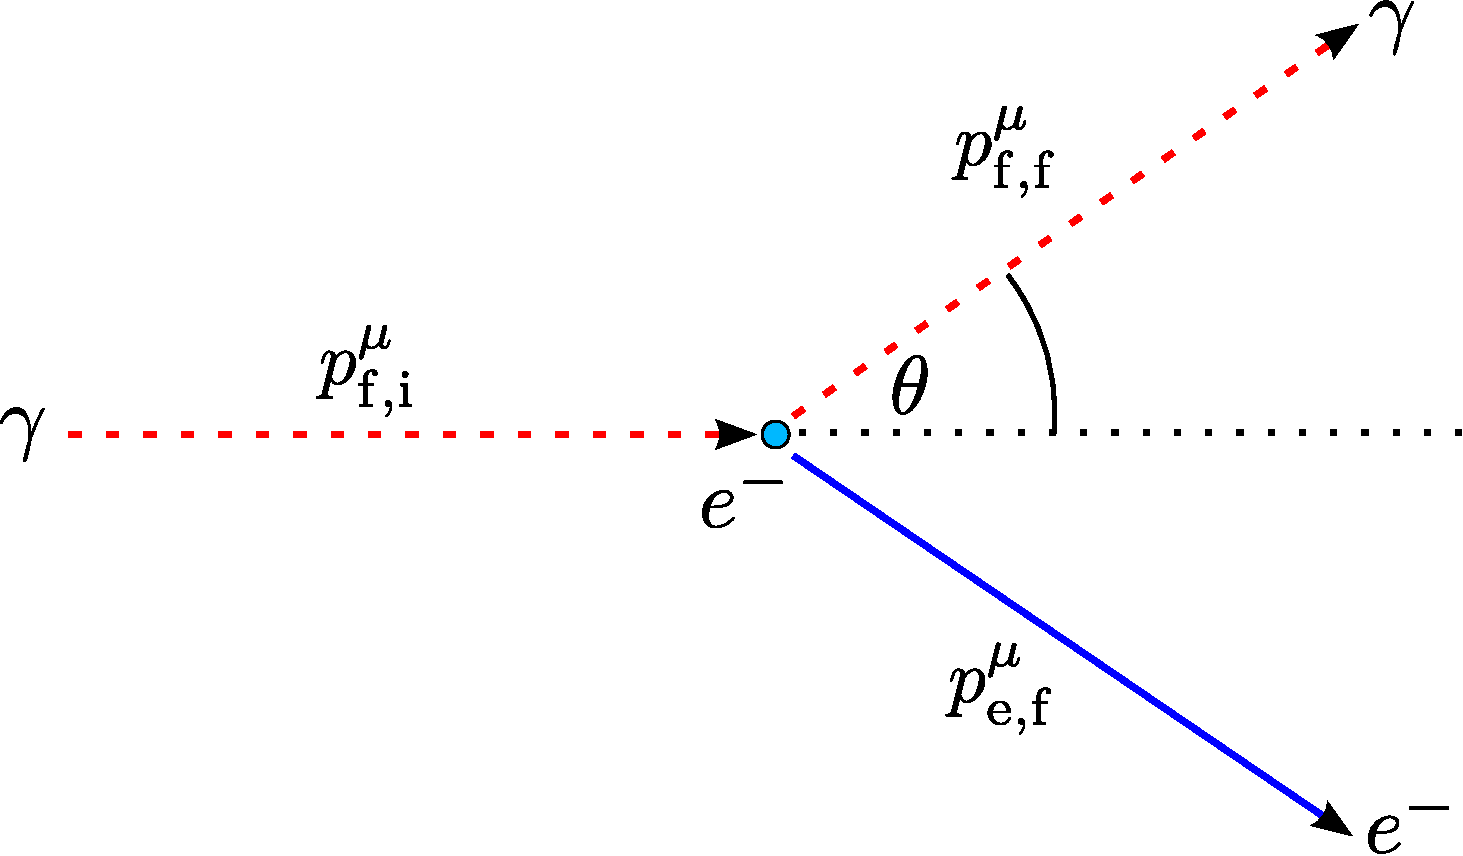
\includegraphics[height=4cm]{fig/fig-Compton.pdf}}
\caption{Scattering por un electr'on, visto desde el SRI com'ovil con el electr'on inicial}
\label{fig:Compton}
\end{figure}
La conservaci'on del 4-momentum (es decir, energ'ia y momentum), en este caso
es:
\begin{equation}
p^\mu_{\rm e,i}+p^\mu_{\rm f,i}=p^\mu_{\rm e,f}+p^\mu_{\rm f,f}.
\end{equation}
Es conveniente reordenar los t'erminos y calcular el escalar correspondiente al
``cuadrado'' del 4-vector correspondiente, de modo que
\begin{eqnarray}
\left( p_{\rm e,i}-p_{\rm e,f}\right)^2 &=&\left( p_{\rm f,f}-p_{\rm
f,i}\right)^2 ,\\
p^2_{\rm e,i}+p^2_{\rm e,f}-2\,p^\mu_{\rm e,i}\,p_\mu^{\rm e,f} &=& p^2_{\rm
f,f}+p^2_{\rm f,i}-2\,p^\mu_{\rm f,i}\,p_\mu^ {\rm f,f},\\
m_{\rm e}^2 c^2+m_{\rm e}^2 c^2-2\left[\frac{E_{\rm e,i}}{c}\frac{E_{\rm e,f}}{c}-\vec{0}\cdot\vec{p}_{\rm e,f}\right] &=&
0+0-2\left[\frac{E_{\rm f,i}}{c}\frac{E_{\rm f,f}}{c}-\vec{p}_{\rm
f,i}\cdot\vec{p}_{\rm f,f}\right] ,\\
m_{\rm e}^2 c^2-m_{\rm e}E_{\rm e,f} &=& -\left[
\frac{\hbar\omega_{\rm i}}{c}\frac{\hbar\omega_{\rm f}}{c}-|\vec{p}_{\rm f,i}||\vec{p}_{\rm f,f}|\cos\theta\right] , \\
m_{\rm e}^2 c^2-m_{\rm e}E_{\rm e,f} &=&
-\frac{\hbar\omega_{\rm i}}{c}\frac{\hbar\omega_{\rm f}}{c}\left(1 -\cos\theta\right) .
\end{eqnarray}
Aqu'i hemos usado que en el SRI com'ovil con el electr'on inicial $p^\mu_{\rm
e,i}=({E_{\rm e,i}}/{c},\vec{0})$, y que para fotones $E_{\rm
f}=|\vec{p}_{\rm f}|c=\hbar\omega$. Ahora reescribiremos la energ'ia $E_{\rm
e,f}$ usando la conservaci'on de la energ'ia:
\begin{eqnarray}
E_{\rm e,i}+E_{\rm f,i}&=&E_{\rm e,f}+E_{\rm f,f}, \\
m_{\rm e}c^2+\hbar\omega_{\rm i} &=&E_{\rm e,f}+\hbar\omega_{\rm f} .
\end{eqnarray}
Entonces, podemos escribir
\begin{eqnarray}
m_{\rm e}^2 c^2-m_{\rm e}\left(m_{\rm e}c^2+\hbar\omega_{\rm i}
-\hbar\omega_{\rm f} \right)  &=&
-\frac{\hbar\omega_{\rm i}}{c}\frac{\hbar\omega_{\rm f}}{c}\left(1 -\cos\theta\right), \\
-m_{\rm e}\hbar\omega_{\rm i} +m_{\rm e}\hbar\omega_{\rm f}   &=&
-\frac{\hbar\omega_{\rm i}}{c}\frac{\hbar\omega_{\rm f}}{c}\left(1 -\cos\theta\right) ,\\
\omega_{\rm f}\left[ m_{\rm e}+\frac{\hbar\omega_{\rm i}}{c^2}\left(1
-\cos\theta\right) \right]   &=& m_{\rm e}\omega_{\rm i} .
\end{eqnarray}
As'i, encontramos que la frecuencia del fot'on emitido en un 'angulo $\theta$ es de la forma
\begin{equation}
\omega_{\rm f}=\frac{\omega_{\rm i}}{\left[ 1+\frac{\hbar\omega_{\rm i}}{m_{\rm
e}c^2}\left(1 -\cos\theta\right) \right] }
\end{equation}
o, equivalentemente, su longitud de onda es
\begin{eqnarray}
\lambda_{\rm f}&=&\lambda_{\rm i}\left[ 1+\frac{\hbar\omega_{\rm i}}{m_{\rm
e}c^2}\left(1 -\cos\theta\right) \right]\\
&=&\lambda_{\rm i}+\frac{2\pi\hbar}{m_{\rm e}c}\left(1 -\cos\theta\right).
\end{eqnarray}
De aqu'i obtenemos directamente la expresi'on para el \textit{cambio de longitud de onda del fot'on}:
\begin{equation}
\Delta \lambda=\frac{h}{m_{\rm e}c}\left(1-\cos\theta\right)=\frac{2h}{m_{\rm e}c}\sin^2\left(\frac{\theta}{2}\right). \label{compton}
\end{equation}
 Desde el punto de vista de una teor'ia corpuscular de la luz, la reducci'on de frecuencia de la radiaci'on emitida es natural debido a que parte de la energ'ia del fot'on inicial es transferida al electr'on (recoil). Por otra parte, este resultado no puede ser entendido en el marco de la teor'ia ondulatoria cl'asica. Compton dedujo y confirm'o experimentalmente (\ref{compton}) en 1922 \cite{Compton23}. El recoil del electr'on fue medido un a\~no m'as tarde por Wilson, usando una c'amara de niebla.
La longitud de Compton del electr'on, ${h}/{m_{\rm e}c}\approx 2,426\times 10^{-12}\,m$.

\item Imposibilidad de emisi'on de un fot'on por un electr'on libre. Ver figura (\ref{fig:no-emision}).
\begin{figure}[h!]
\centerline{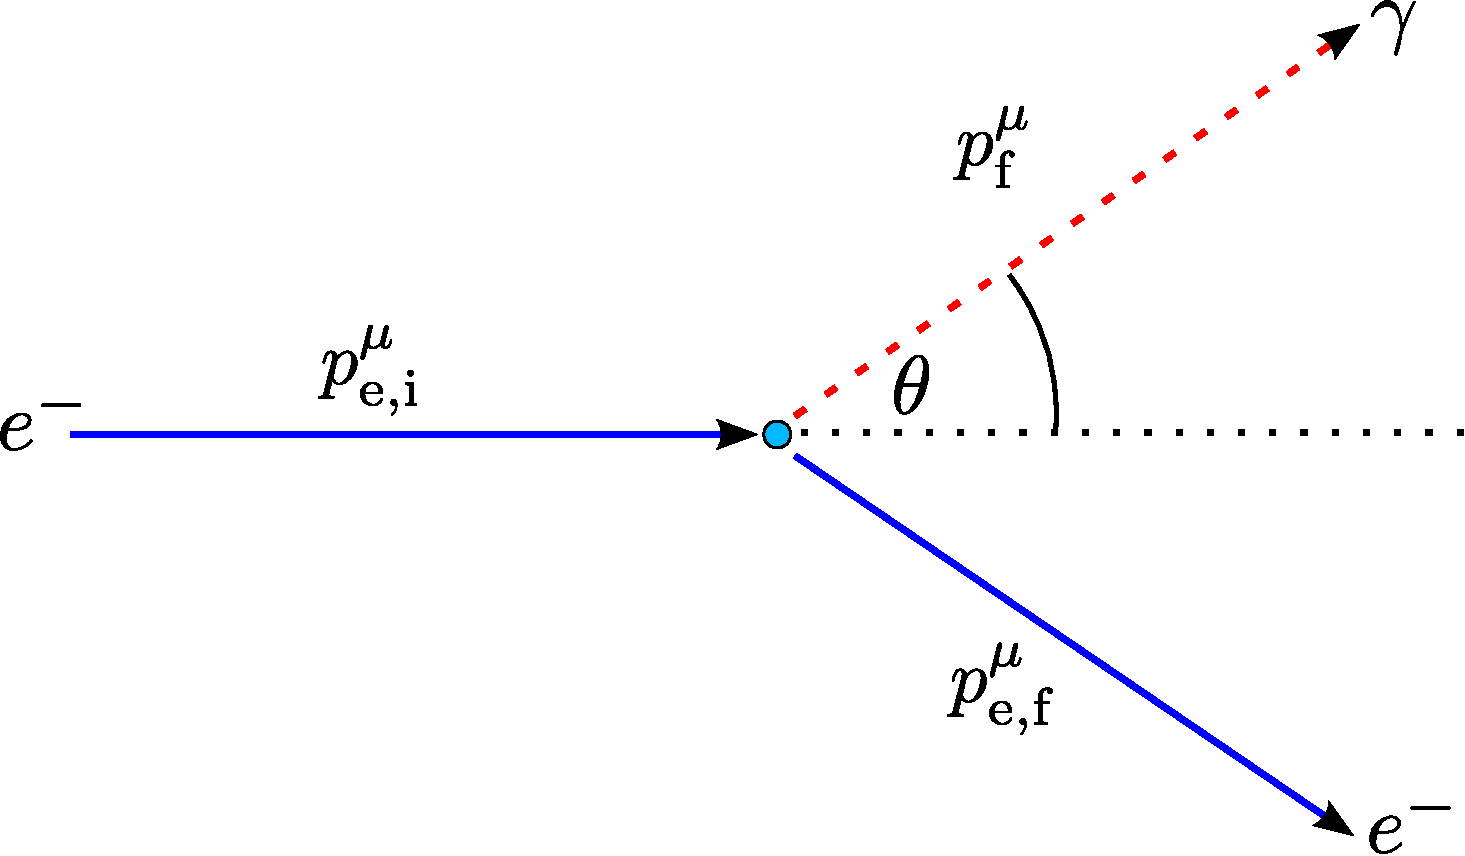
\includegraphics[height=4cm]{fig/fig-no-emision.pdf}}
\caption{Diagrama para la (prohibida) emisi'on de un fot'on por un electr'on libre.}
\label{fig:no-emision}
\end{figure}

\begin{equation}
p^\mu_{\rm e,i}=p^\mu_{\rm e,f}+p^\mu_{\rm f}.
\end{equation}
\begin{eqnarray}
\left( p_{\rm e,i}-p_{\rm f}\right)^2 &=&\left( p_{\rm e,f}\right)^2 ,\\
p^2_{\rm e,i}+p^2_{\rm \rm f}-2\,p^\mu_{\rm e,i}\,p_{\mu, \rm f} &=& p^2_{\rm e,f} ,\\
m_{\rm e}^2 c^2+0-2\,p^\mu_{\rm e,i}\,p_{\mu, \rm f} &=& m_{\rm e}^2 c^2.
\end{eqnarray}
Por lo tanto,
\begin{equation}
p^\mu_{\rm e,i}\,p_{\mu, \rm f}=0.\label{sorry}
\end{equation}
En el sistema en reposo del electr'on inicial, tenemos
\begin{equation}
p^\mu_{\rm e,i}\,p_{\mu, \rm f}=\frac{E_{\rm e,i}}{c}\frac{E_{\rm f}}{c} =m_{\rm
e}E_{\rm f},
\end{equation}
de modo que (\ref{sorry}) implica que $E_{\rm f}=0$ y por tanto $p^\mu_{\rm
f}=0$, es decir, que no hay fot'on!.
\end{itemize}
